% Hypothesis
% \begin{itemize}
%     \item Separability is important
%     \begin{itemize}
%         \item Separation sets
%         \item All positive network
%     \end{itemize}
%     \item Controlling separability enhances the network
%     \begin{itemize}
%         \item Depth
%         \item Dead units
%         \item Zero init
%         \item Moons data shattering
%     \end{itemize}
%     \item Separability works in real world
%     \begin{itemize}
%         \item Toy Cifar
%         \item SimpNet
%         \item ULMfit
%         \item Fixup
%     \end{itemize}
% \end{itemize}

\section{Experiments and Results}\label{sec:experiments}
After presenting the separability constraints, we test our formulation in an example of a \ReLU-based network (of depth $d=50$, and fixed layer width $N_k=4$), specially targeted to: 
\begin{enumerate}
    \item fail to trivial accuracy values with \ReLU and batchnorm.
    \item exhibit the highlighted issues that DNN experience: dying neurons, vanishing gradient, and to some extent exploding gradient.
    \item is manageable enough to relate to analytical results presented previously.
\end{enumerate}
Experimentation was done over two datasets: the \moons dataset (for \emph{toying}) and the \texttt{CIFAR-10} to test in a more realistic setting involving (a CNN with $5\times 5$ kernels with padding to preserve image size), using \texttt{Keras} and \texttt{TensorFlow}.
\\\\
Within the \moons dataset we sampled $100$ points ($85$ for training and $15$). As hyper-parameters, we used learning rates $\gamma \in \{0.01, 0.001, 0.0001\}$, a batch size $bs = 85$, to ensure \emph{fairness} for \SepUnit.  For testing, the loss functional $\mathcal{L}$ in equation \ref{eq:constraintLossFunctional}  was chosen to be the cross-entropy as presented in \cite{LeCun06atutorial}, introducing constraint loss parameter $\lambda = 0.01$ using $T = 2000$ epochs. 
\\\\
Due to the fact that \cifar is a much larger dataset, choosing hyper-parameters for experimentation were chosen empirically. Learning rates are \emph{smaller} than the ones used for \moons: $\gamma \in \{0.001, 0.0005, 0.0001 \}$, while extending experimentation to two batch sizes: $64$ and $128$.  Constraint trade-off parameter $\lambda$ was tuned using: $10^{-5},10^{-3}$ and $1$ values, and for the sake of speed we set the number of epochs to $T = 500$.
\\\\
In matters of \emph{initialization} two schemes were tested: the \emph{Glorot Uniform Scheme} implemented in \texttt{Keras} following (see \cite{Glorot10Initialization} for the technical details) and \emph{zero initialization} consisting in setting weights and biases to zero. 

\subsection{Visualization}\label{subsec:visualization}


In order to understand the effect that separability has we use the \moons dataset. We train 50x4 network on the moons dataset with batch size equal to the entire training set for each of our proposals plus \ReLU and \ReLUBN, which we show in Figures \ref{fig:moonsReLU},\ref{fig:moonsReLUBN},\ref{fig:moonsLayerwise},\ref{fig:moonsUnitwise},\ref{fig:moonsPointwise} and \ref{fig:moonsUnitpointwise}. The first column shows the data space with the partitions performed by the first layer in the native space. The blue lines show the separating plane whereas the gray zone accounts for the zero area of each of the 4 units. Next to it, we show the 4th, 25th and classification layers in pairs (one plot for pair of coordinates), to see how the data evolves as in goes through the network. Finally, the last column shows the output surface of the network in the original data space. 

\begin{figure*}
  \centering
  \parbox{\textwidth}{
    \parbox{.195\textwidth}{%
      \subcaptionbox{Input layer}{\includegraphics[width=\hsize]{img/toy/relu/conv2d_1-0.pdf}}
    }
    % \hskip1em
    \parbox{.195\textwidth}{%
      \subcaptionbox{4th layer}{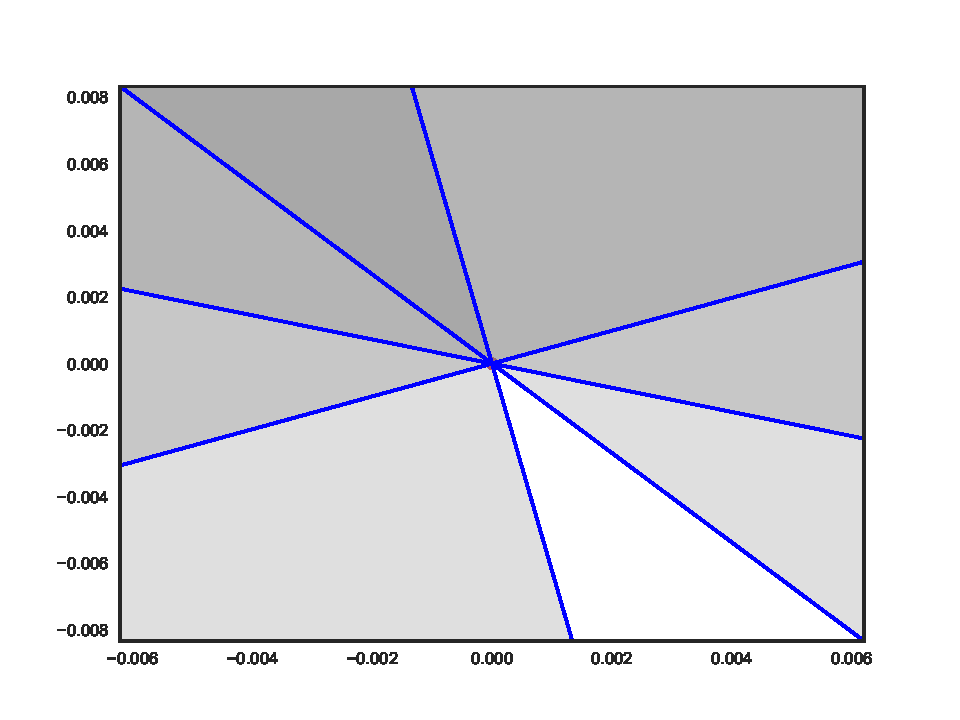
\includegraphics[width=\hsize]{img/toy/relu/conv2d_4-0.pdf}}
    %   \vskip1em
      \subcaptionbox{4th layer}{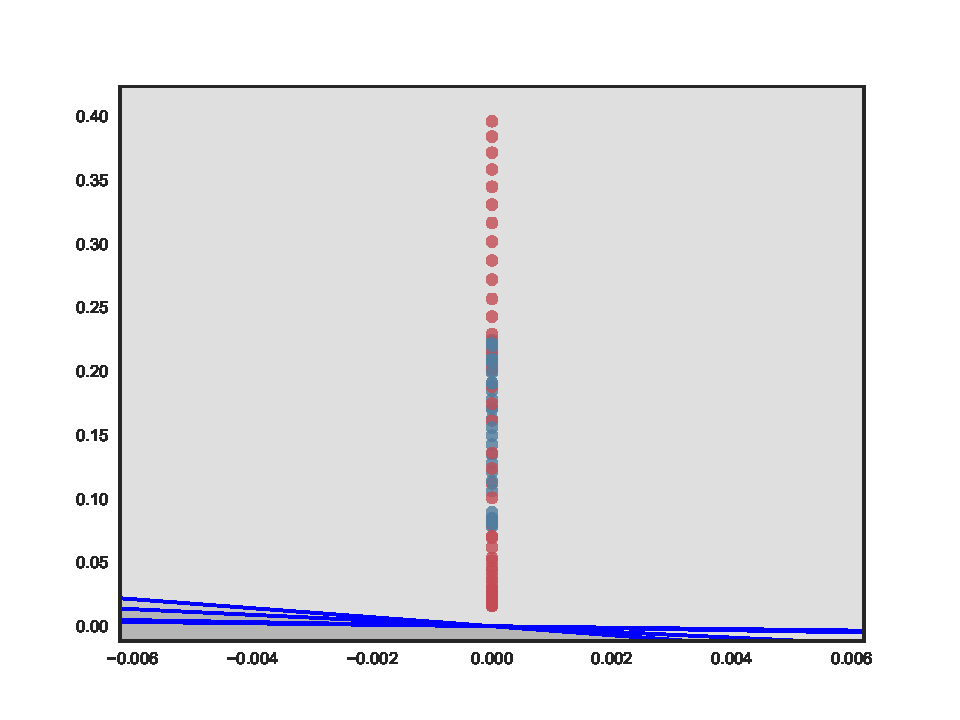
\includegraphics[width=\hsize]{img/toy/relu/conv2d_4-2.pdf}} 
    }
    % \hskip1em
    \parbox{.195\textwidth}{%
      \subcaptionbox{25th layer}{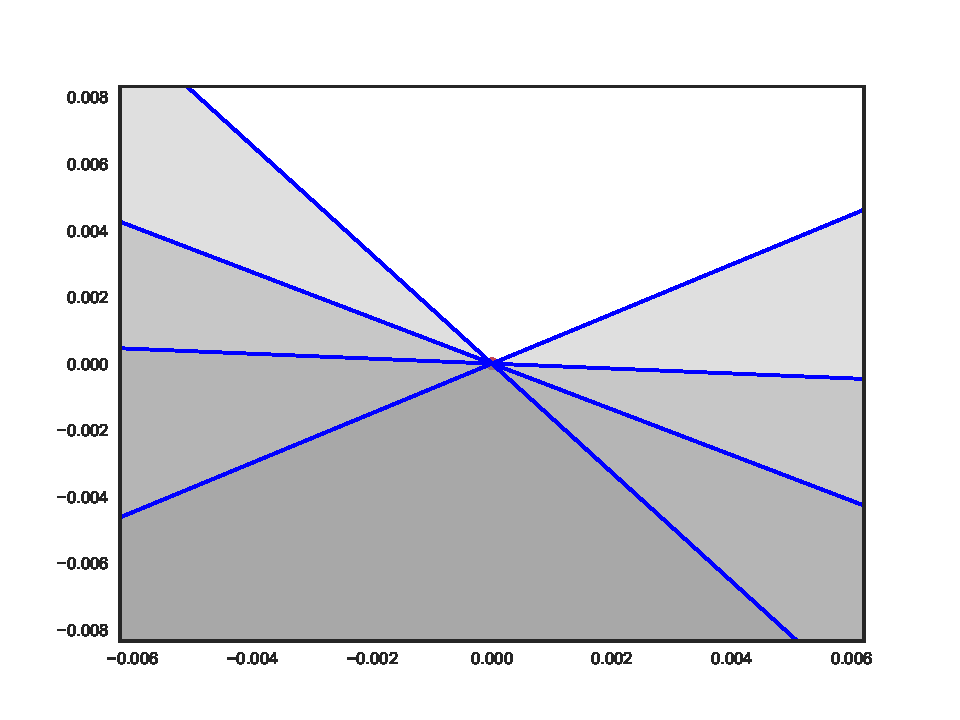
\includegraphics[width=\hsize]{img/toy/relu/conv2d_25-0.pdf}}
    %   \vskip1em
      \subcaptionbox{25th layer}{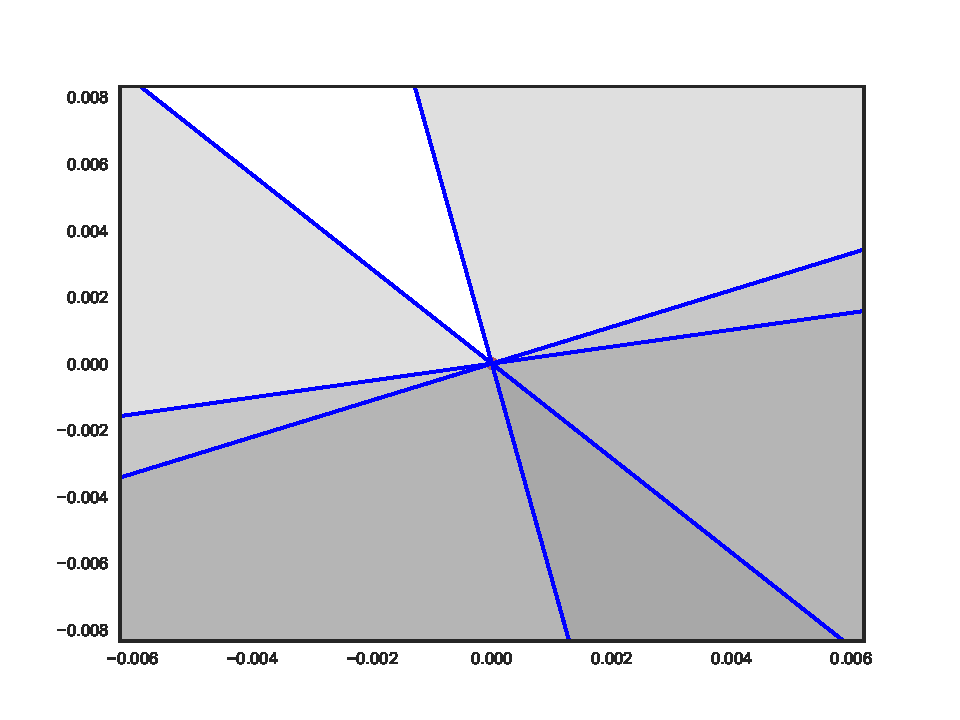
\includegraphics[width=\hsize]{img/toy/relu/conv2d_25-2.pdf}} 
    }
    % \hskip1em
    \parbox{.195\textwidth}{%
      \subcaptionbox{Classification layer}{\includegraphics[width=\hsize]{img/toy/relu/dense_1-0.pdf}}
    %   \vskip1em
      \subcaptionbox{Classification layer}{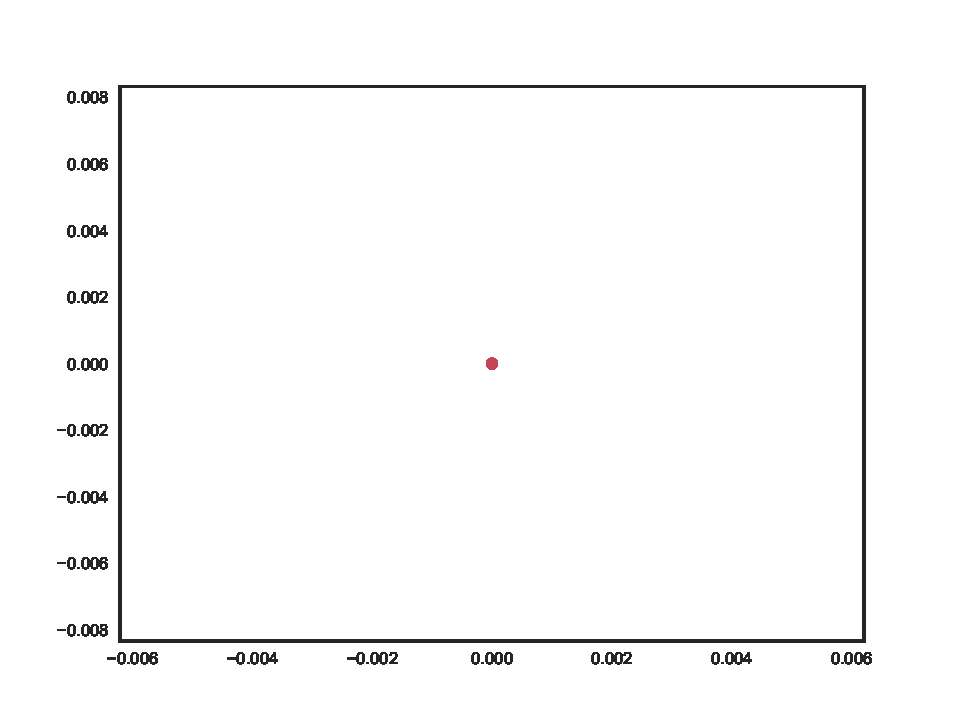
\includegraphics[width=\hsize]{img/toy/relu/dense_1-2.pdf}} 
    }
    % \hskip1em
    \parbox{.195\textwidth}{%
      \subcaptionbox{Output}{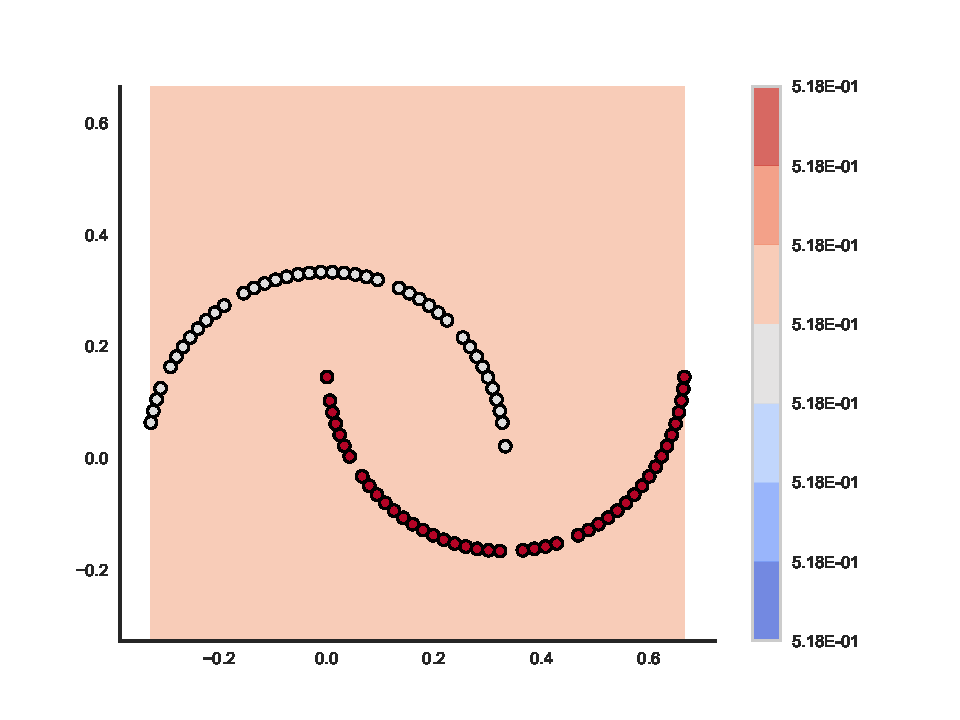
\includegraphics[width=\hsize]{img/toy/relu/output.pdf}}
    }
  }
  \caption{ReLU}
    \label{fig:moonsReLU}
\end{figure*}


Notice how the gradient has changed the separation performed by \ReLU in Figure \ref{fig:moonsReLU} at the input layer (a), but it fails to find a proper representation of use for the upper layers ((b), (c), (d)), so starting from the middle of the network it sends the entire dataset to zero. This leads to the total failure to output anything useful (j) which will make difficult to get any kind of \emph{useful} gradient in order to escape from this situation. We argue that this is due the fact that the lower layers (b) are breaking the \emph{topological structure} of the classes of the dataset, making the gradient of the respective layers so \emph{unrelated} with the original structure which fails in fixing the unsuitable partition generated by the random initialization. We relate this phenomena with the lack of smoothness over the transition across layers causing lack of \emph{intuitive} separation, first described in \cite{HauserAsok}. If the transition between the layers is too harsh, mostly due sending too much points to zero due dead units or \emph{overlapping} dead units (one unit sends part of the data to zero whereas the units following them send the rest) the gradient resulting will be unable to traspass the truncations and reach the lower layers which are the ones which are messing it.

\begin{figure*}
  \centering
  \parbox{\textwidth}{
    \parbox{.195\textwidth}{%
      \subcaptionbox{Input layer}{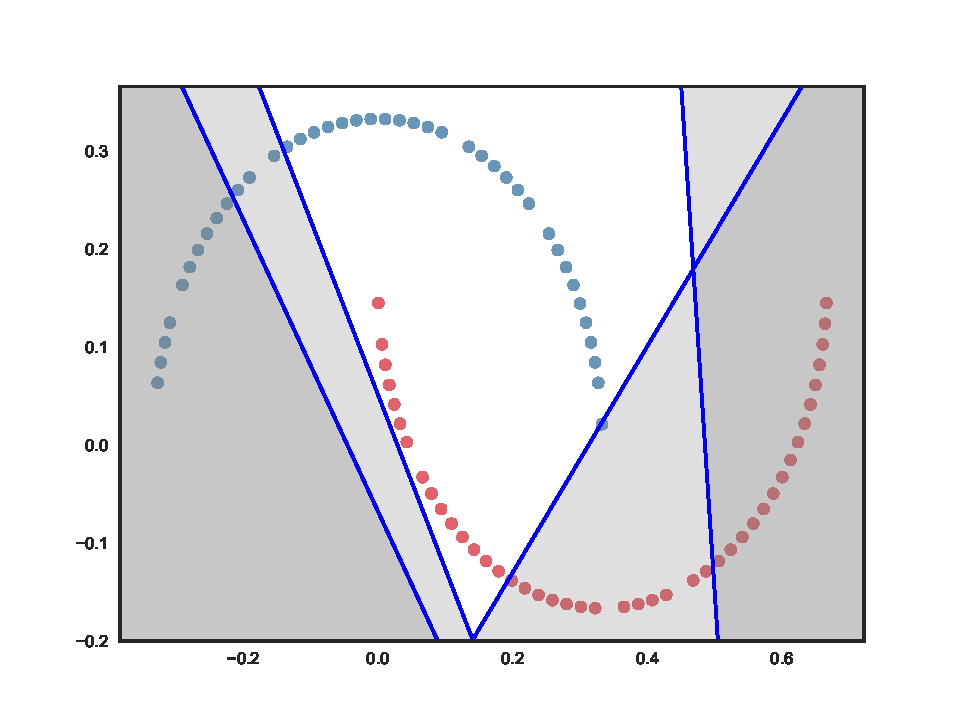
\includegraphics[width=\hsize]{img/toy/relu-bn/conv2d_1-0.pdf}}
    }
    % \hskip1em
    \parbox{.195\textwidth}{%
      \subcaptionbox{4th layer}{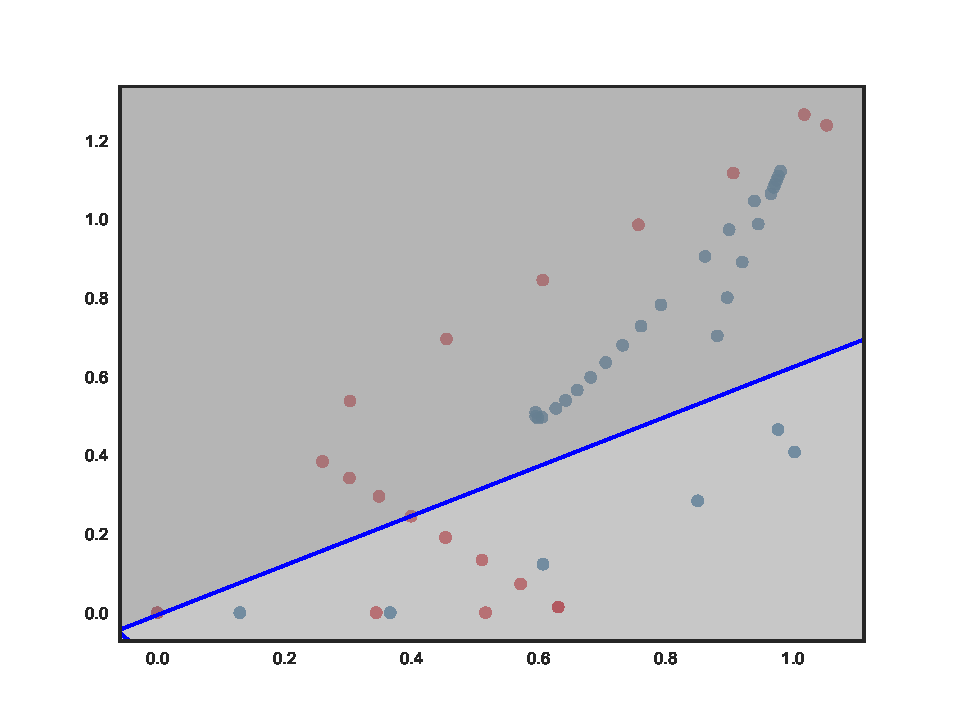
\includegraphics[width=\hsize]{img/toy/relu-bn/conv2d_4-0.pdf}}
    %   \vskip1em
      \subcaptionbox{4th layer}{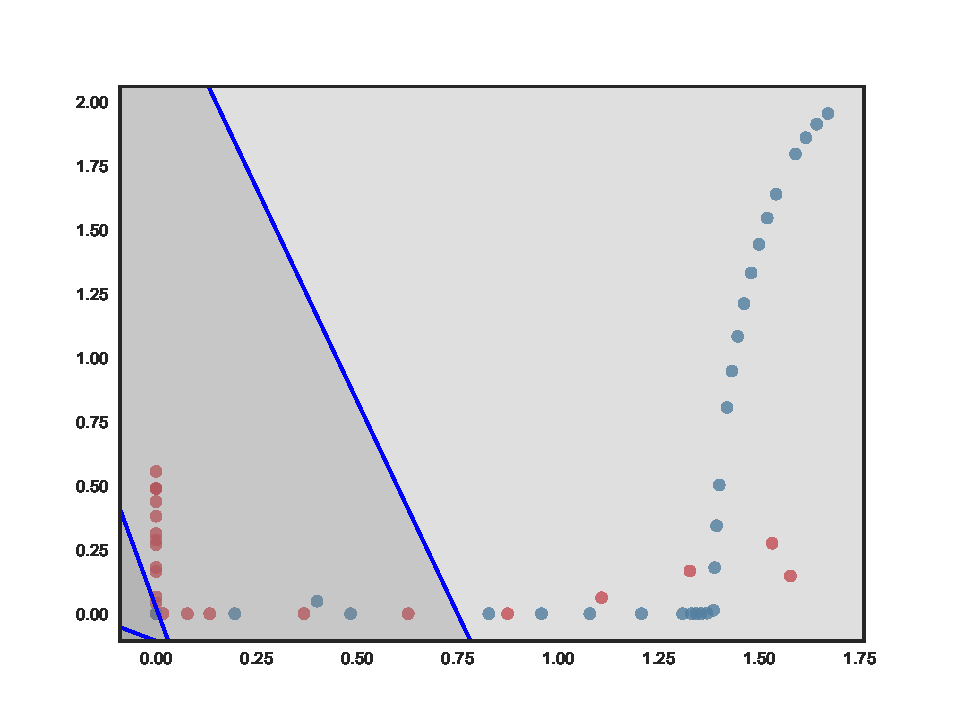
\includegraphics[width=\hsize]{img/toy/relu-bn/conv2d_4-2.pdf}}
    }
    % \hskip1em
    \parbox{.195\textwidth}{%
      \subcaptionbox{25th layer}{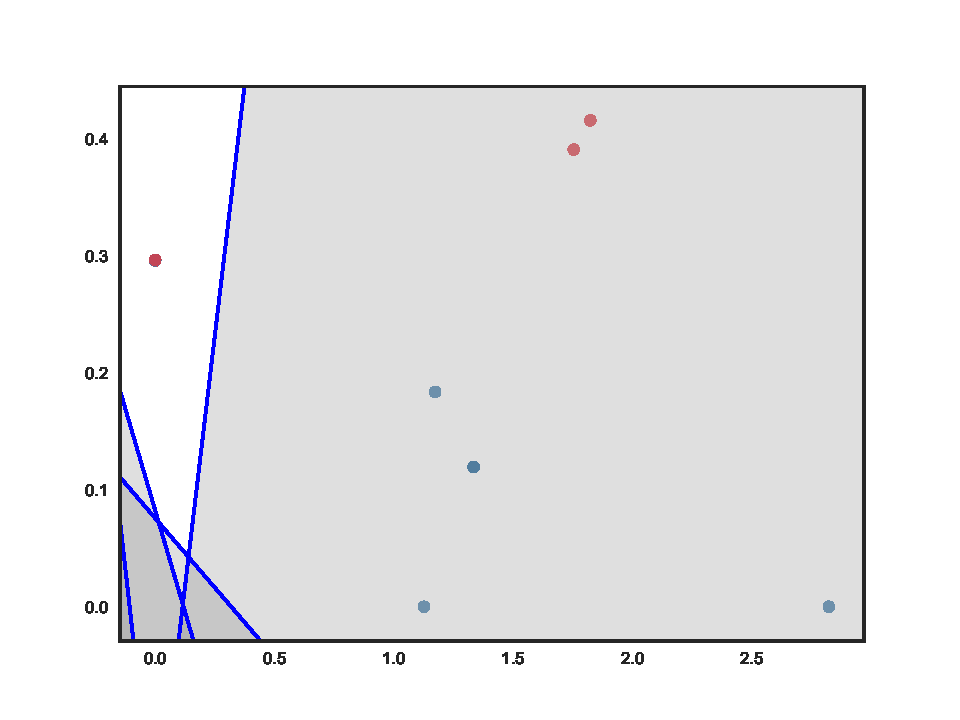
\includegraphics[width=\hsize]{img/toy/relu-bn/conv2d_25-0.pdf}}
    %   \vskip1em
      \subcaptionbox{25th layer}{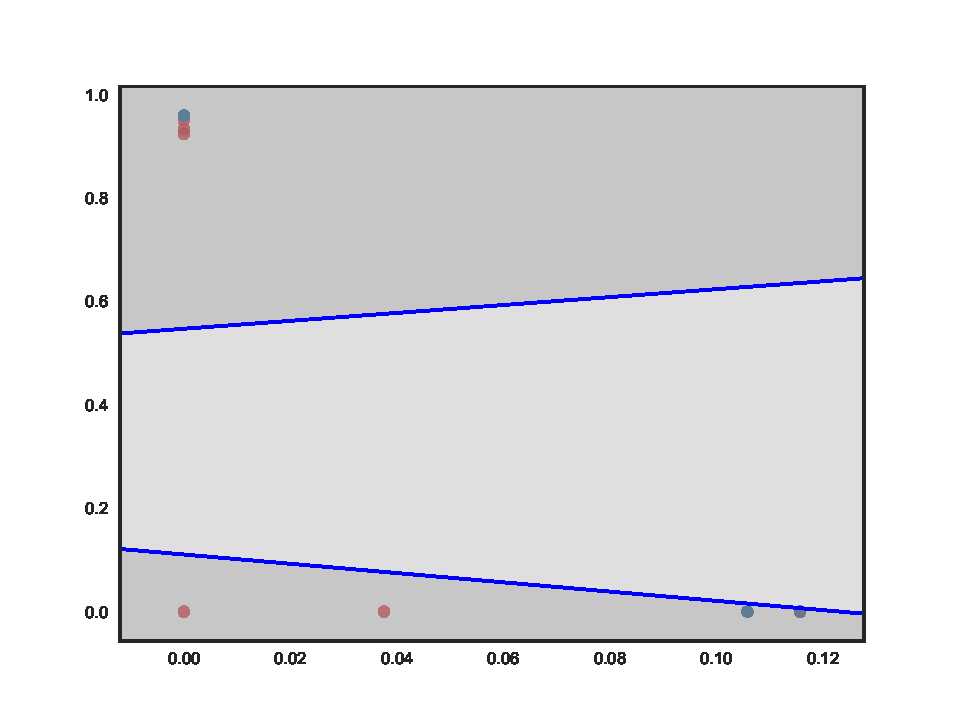
\includegraphics[width=\hsize]{img/toy/relu-bn/conv2d_25-2.pdf}} 
    }
    % \hskip1em
    \parbox{.195\textwidth}{%
      \subcaptionbox{}{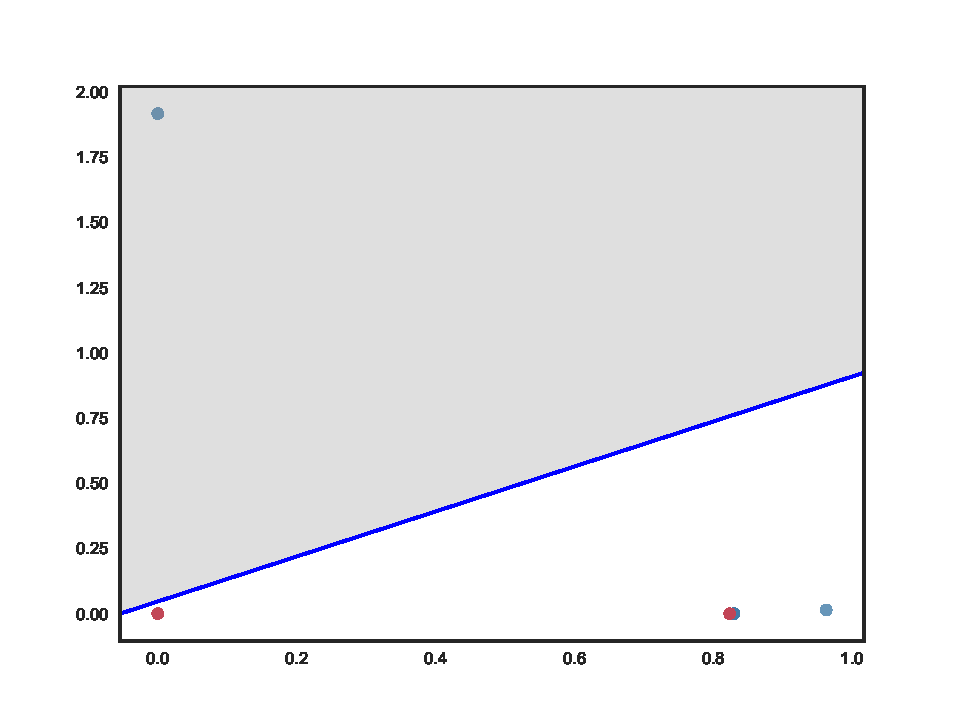
\includegraphics[width=\hsize]{img/toy/relu-bn/dense_1-0.pdf}}
    %   \vskip1em
      \subcaptionbox{}{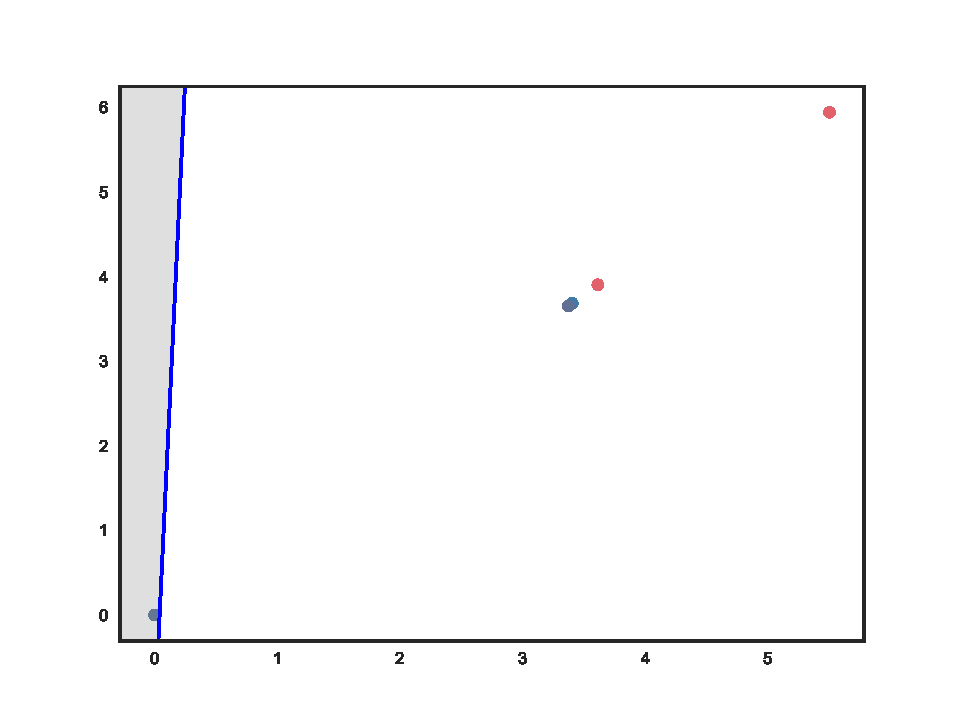
\includegraphics[width=\hsize]{img/toy/relu-bn/dense_1-2.pdf}} 
    }
    % \hskip1em
    \parbox{.195\textwidth}{%
      \subcaptionbox{Output}{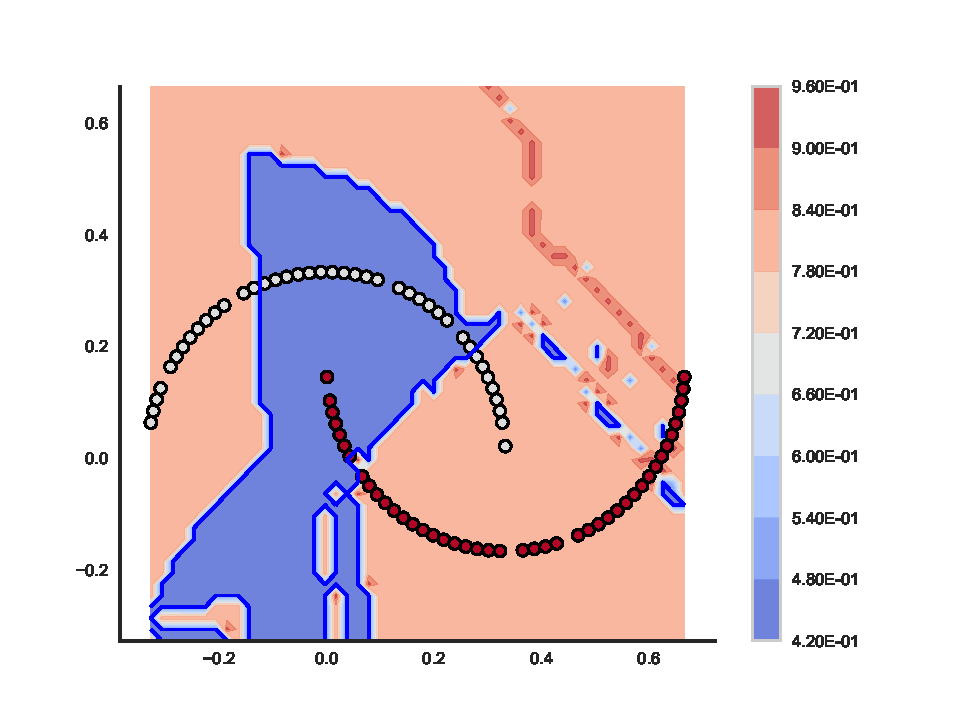
\includegraphics[width=\hsize]{img/toy/relu-bn/output.pdf}}
    }
  }
  \caption{\ReLUBN}
    \label{fig:moonsReLUBN}
\end{figure*}

\ReLUBN fares a bit better since it is able to pull the data out of zero, as we can see in the upper layers ((d), (e), (f), (g)), yet it is still unable to preserve the \emph{topological structure} like \ReLU, which ultimately leads to \emph{data shattering} \cite{dataShattering} and \emph{mezcla topologica}. This generates very strange outputs which we can see in (h) whose gradients fail again to provide hints to the lower layers to fix the topological structure of the network. 

\begin{figure*}
  \centering
  \parbox{\textwidth}{
    \parbox{.195\textwidth}{%
      \subcaptionbox{Input layer}{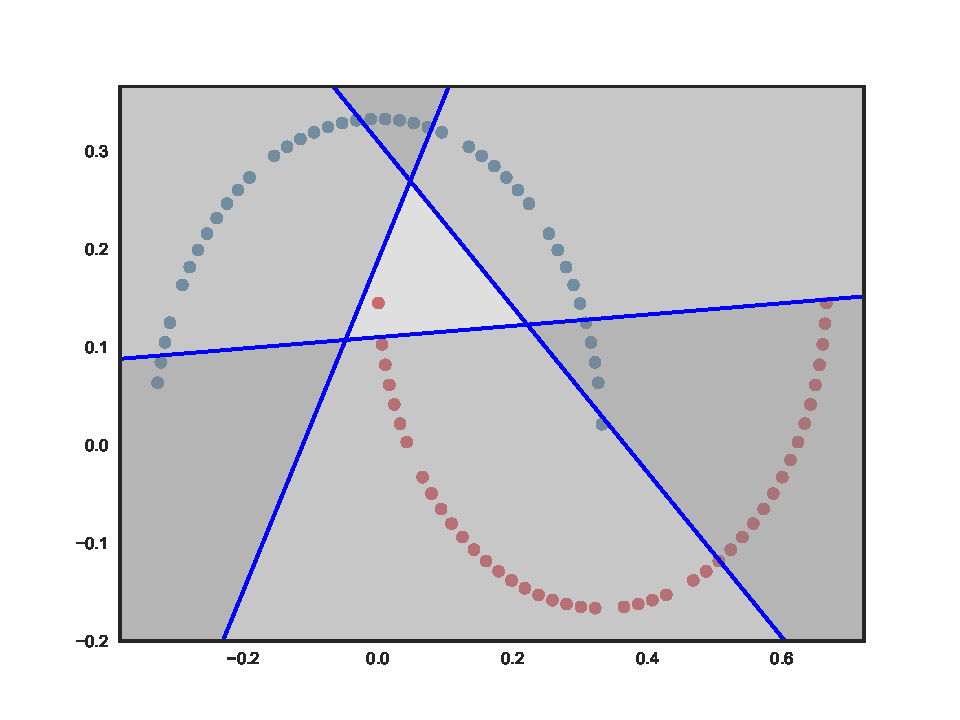
\includegraphics[width=\hsize]{img/toy/layerwise/conv2d_1-0.pdf}}
    }
    % \hskip1em
    \parbox{.195\textwidth}{%
      \subcaptionbox{4th layer}{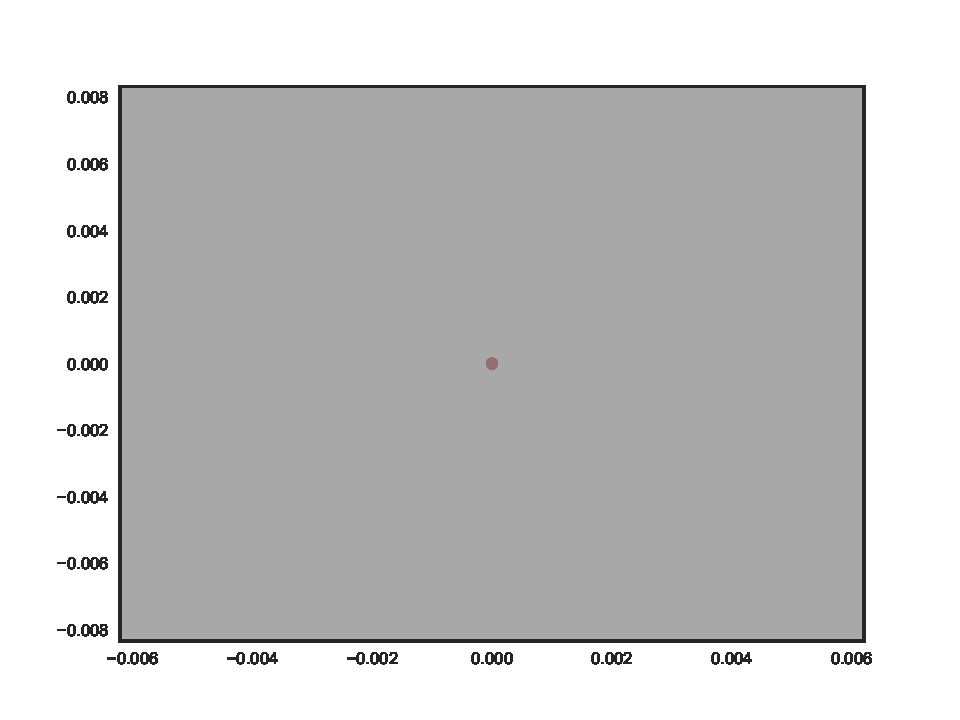
\includegraphics[width=\hsize]{img/toy/layerwise/conv2d_4-0.pdf}}
    %   \vskip1em
      \subcaptionbox{4th layer}{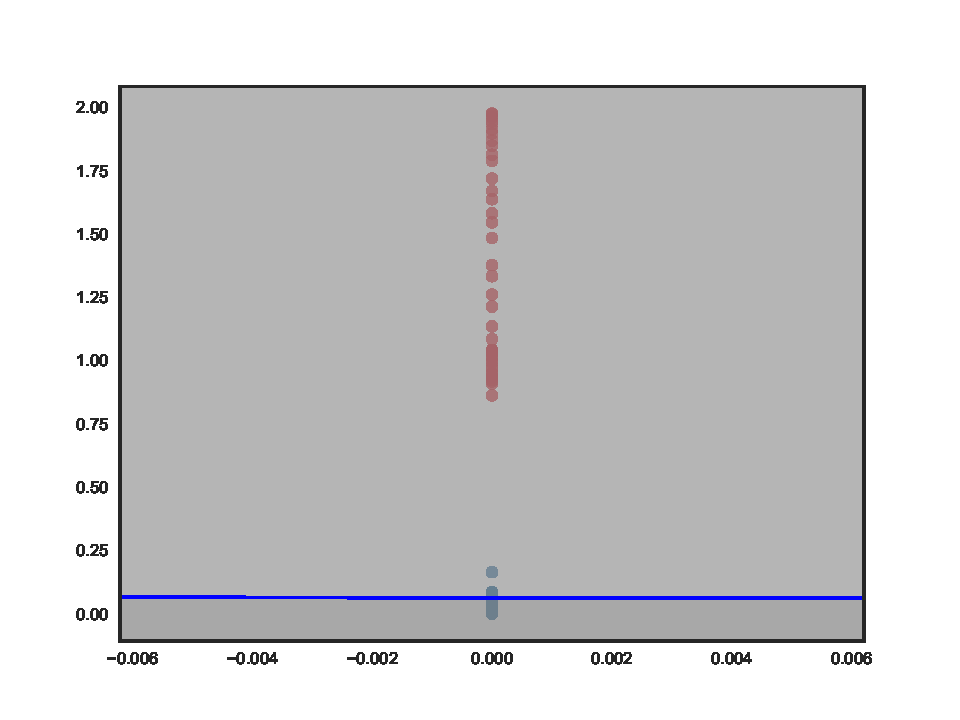
\includegraphics[width=\hsize]{img/toy/layerwise/conv2d_4-2.pdf}} 
    }
    % \hskip1em
    \parbox{.195\textwidth}{%
      \subcaptionbox{25th layer}{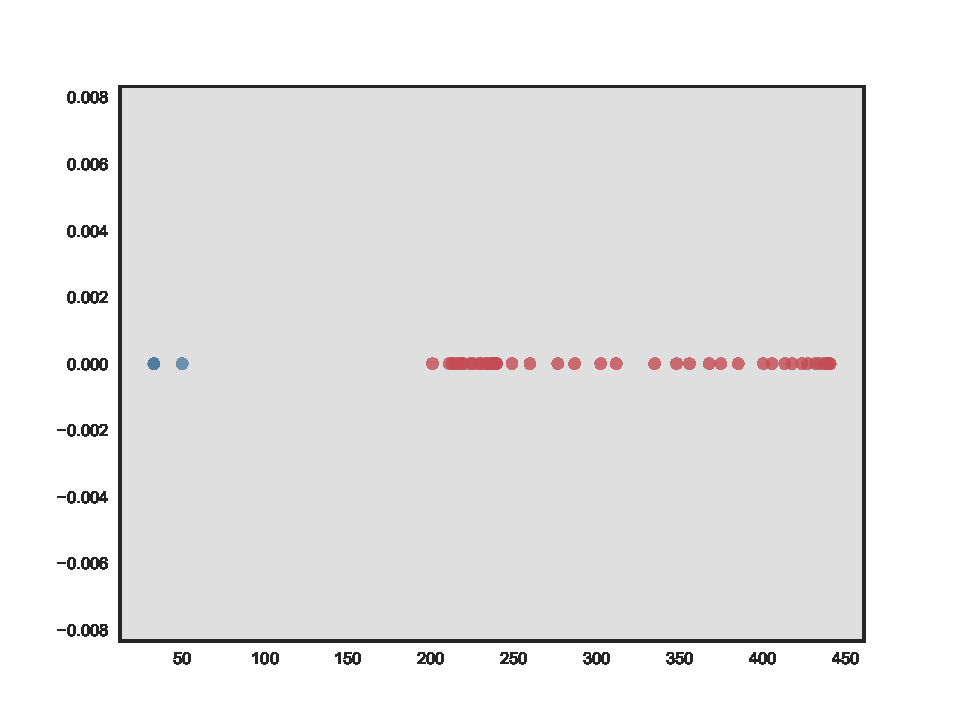
\includegraphics[width=\hsize]{img/toy/layerwise/conv2d_25-0.pdf}}
    %   \vskip1em
      \subcaptionbox{25th layer}{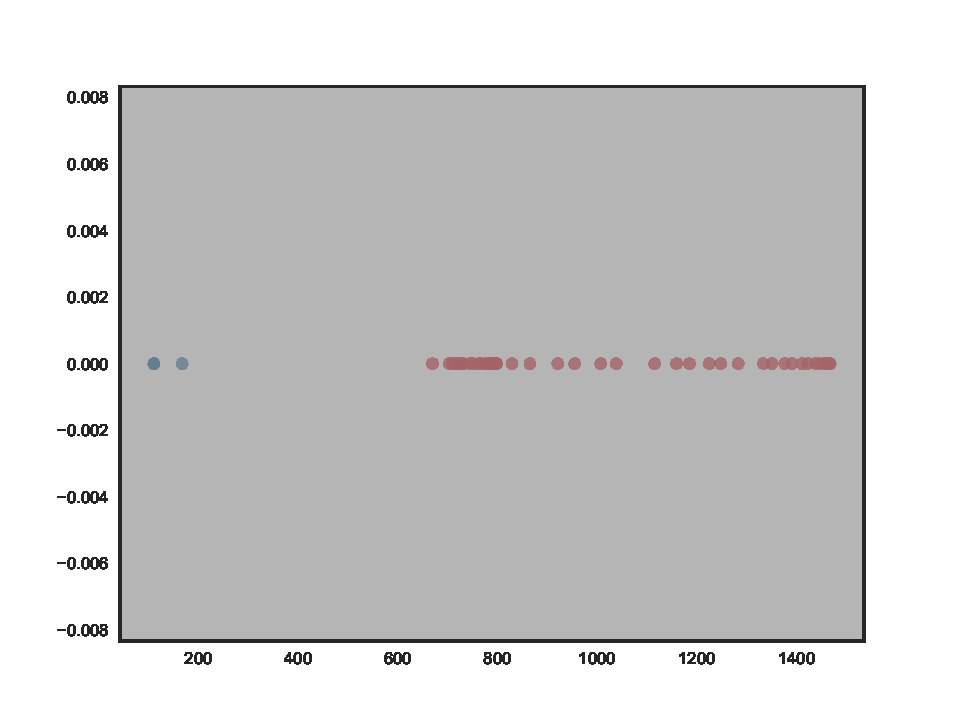
\includegraphics[width=\hsize]{img/toy/layerwise/conv2d_25-2.pdf}} 
    }
    % \hskip1em
    \parbox{.195\textwidth}{%
      \subcaptionbox{Classification layer}{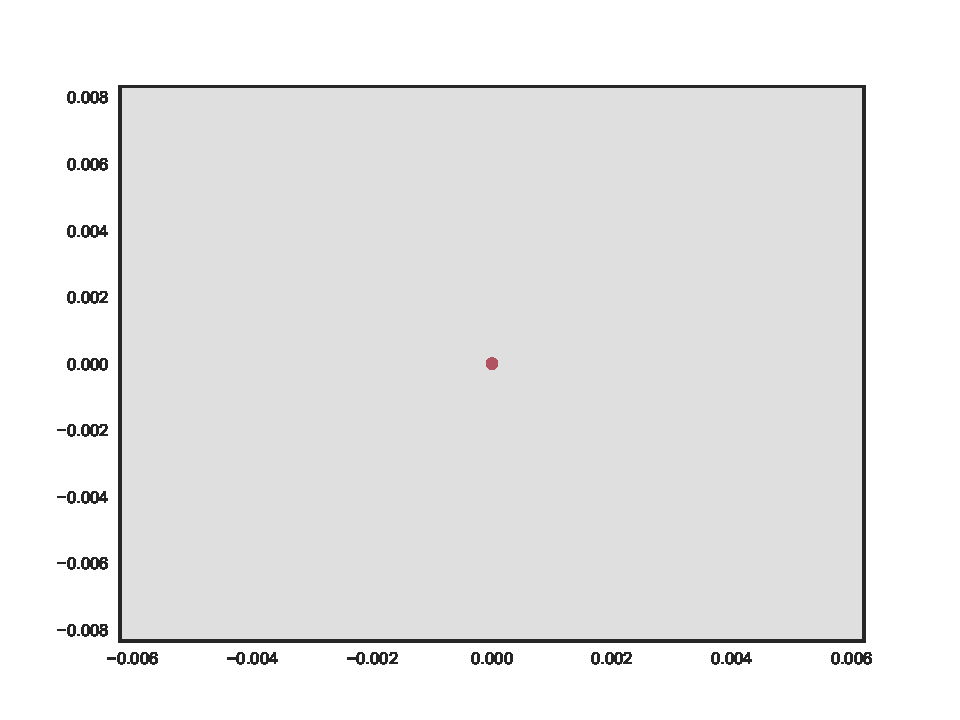
\includegraphics[width=\hsize]{img/toy/layerwise/dense_1-0.pdf}}
    %   \vskip1em
      \subcaptionbox{Classification layer}{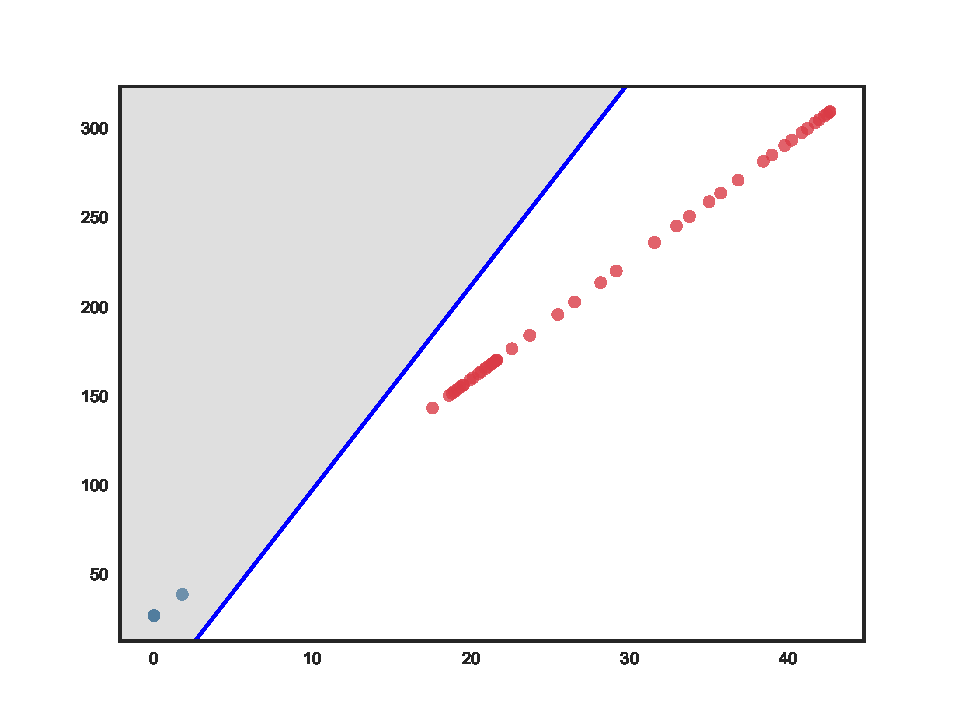
\includegraphics[width=\hsize]{img/toy/layerwise/dense_1-2.pdf}} 
    }
    % \hskip1em
    \parbox{.195\textwidth}{%
      \subcaptionbox{Output}{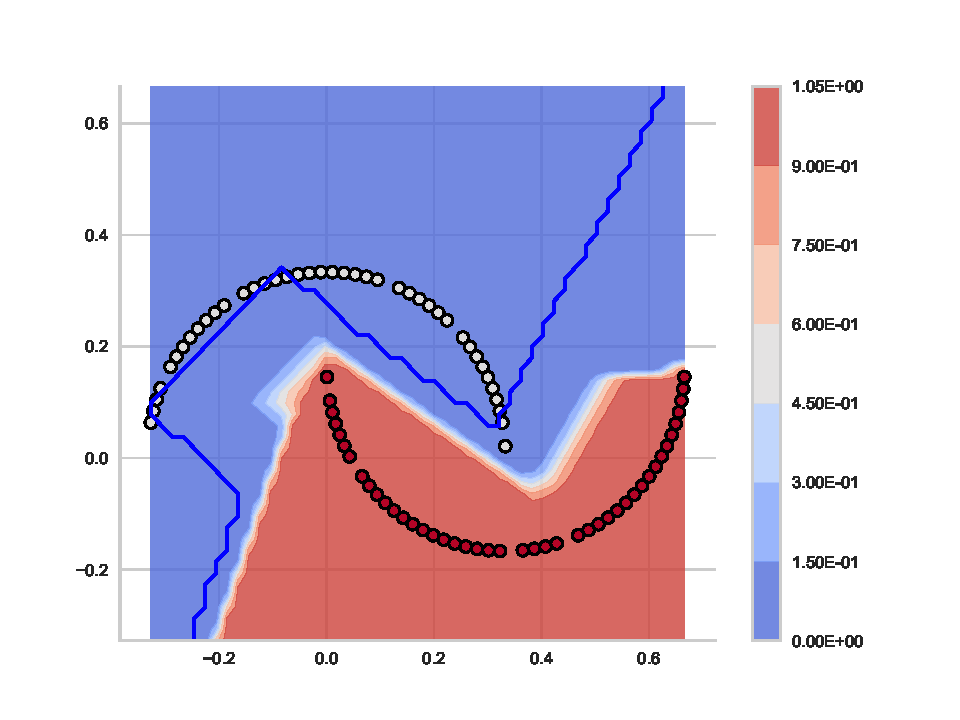
\includegraphics[width=\hsize]{img/toy/layerwise/output.pdf}}
    }
  }
    \caption{\SepLayer}
    \label{fig:moonsLayerwise}
\end{figure*}


In the other hand, our relaxed version of our proposal \SepLayer, see Figure \ref{fig:moonsLayerwise}, is able to solve the problem (h). We find how is able to propagate the information needed for the lower layers to perform the separation, so we can see at (k) how the separating planes are much better placed, so by the bottom layers (c) the problem is already solved and the rest of layers simply forward upwards ((d), (e)). Note how as our formulation is relaxed from \SepUnit we allow are redundant and dead units. Nootice how the entire space is colored in different shades of gray, showing how at (d) least one unit is effectively operating in linear mode, thus showing how in certain situations like the mentioned before affine transforms might be useful \cite{resnet}, \cite{batchnormAffine}. This indicates the role of the upper layers on forwarding the already found solution. 

\begin{figure*}
  \centering
     % Unitwise
  \parbox{\textwidth}{
    \parbox{.195\textwidth}{%
      \subcaptionbox{Input layer}{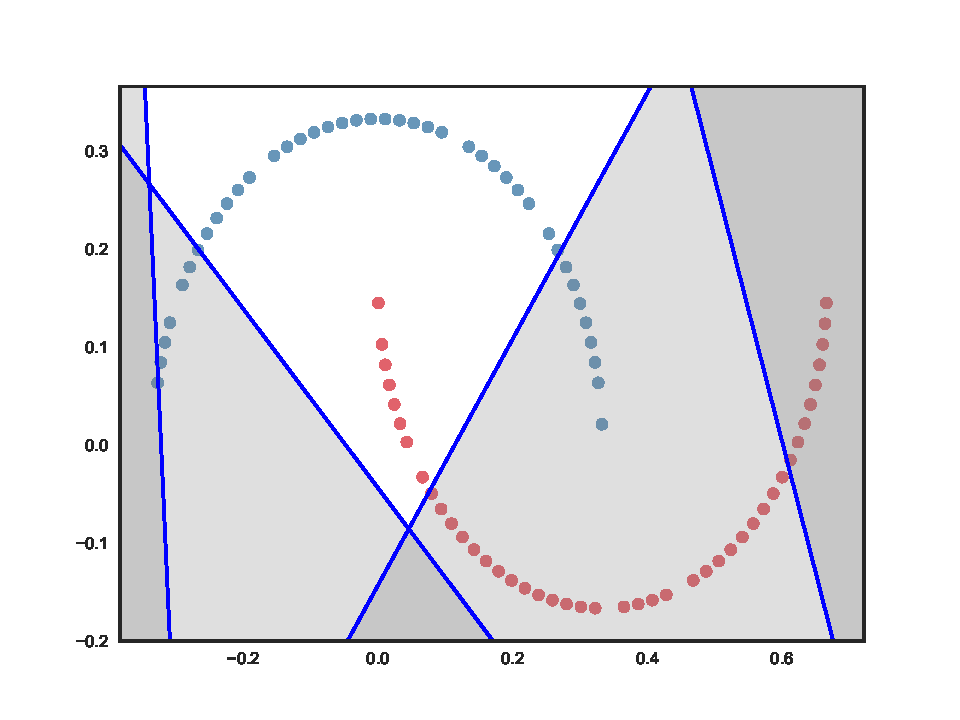
\includegraphics[width=\hsize]{img/toy/unitwise/conv2d_1-0.pdf}}
    }
    % \hskip1em
    \parbox{.195\textwidth}{%
      \subcaptionbox{4th layer}{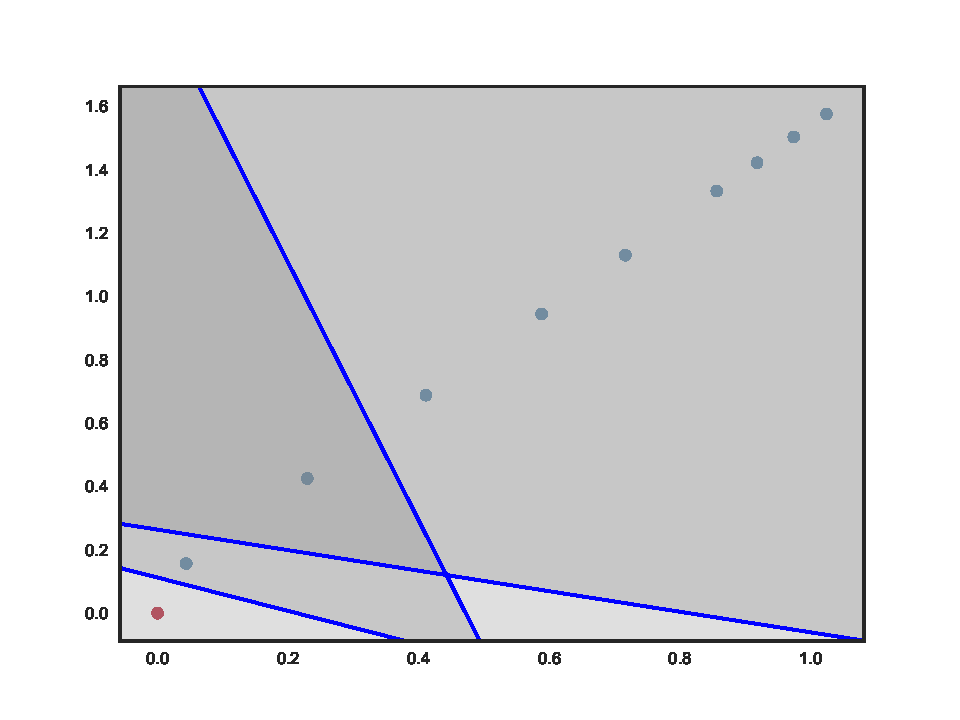
\includegraphics[width=\hsize]{img/toy/unitwise/conv2d_4-0.pdf}}
    %   \vskip1em
      \subcaptionbox{4th layer}{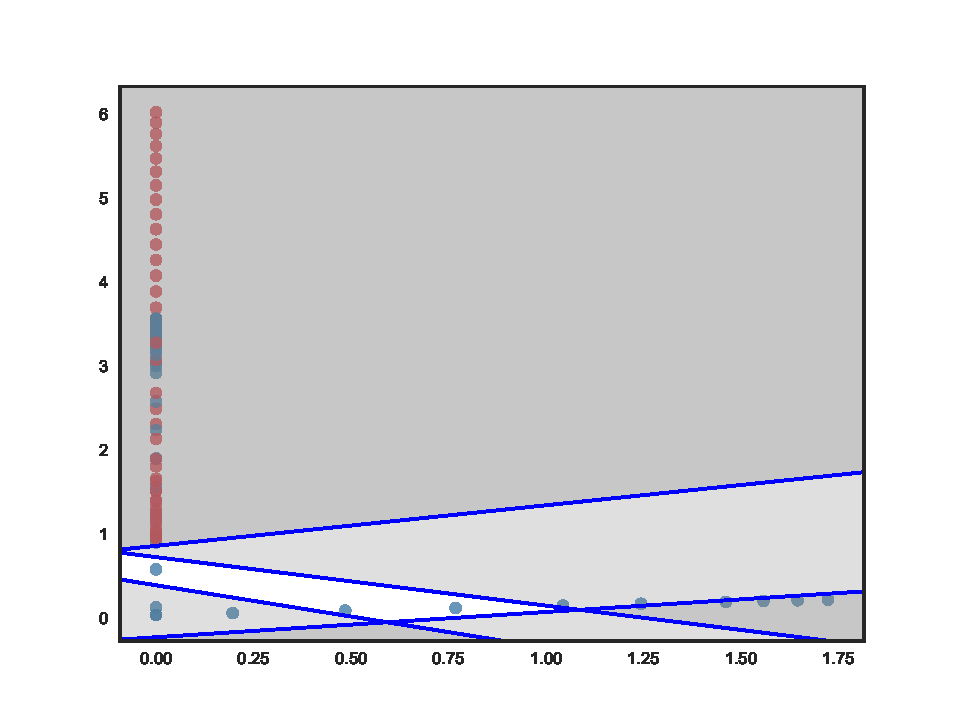
\includegraphics[width=\hsize]{img/toy/unitwise/conv2d_4-2.pdf}} 
    }
    % \hskip1em
    \parbox{.195\textwidth}{%
      \subcaptionbox{25th layer}{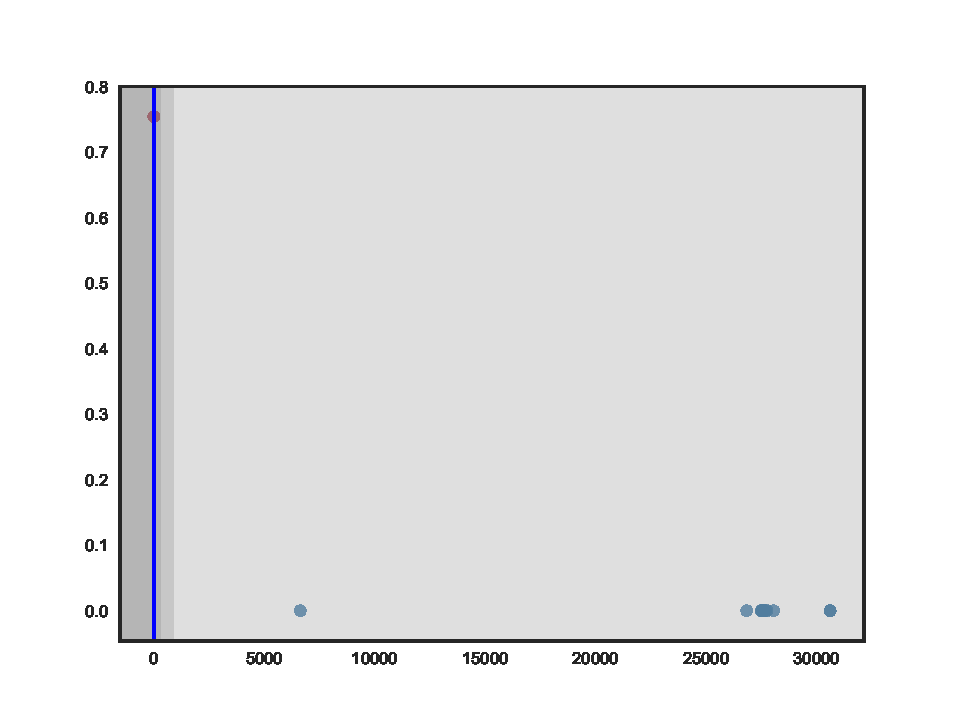
\includegraphics[width=\hsize]{img/toy/unitwise/conv2d_25-0.pdf}}
    %   \vskip1em
      \subcaptionbox{25th layer}{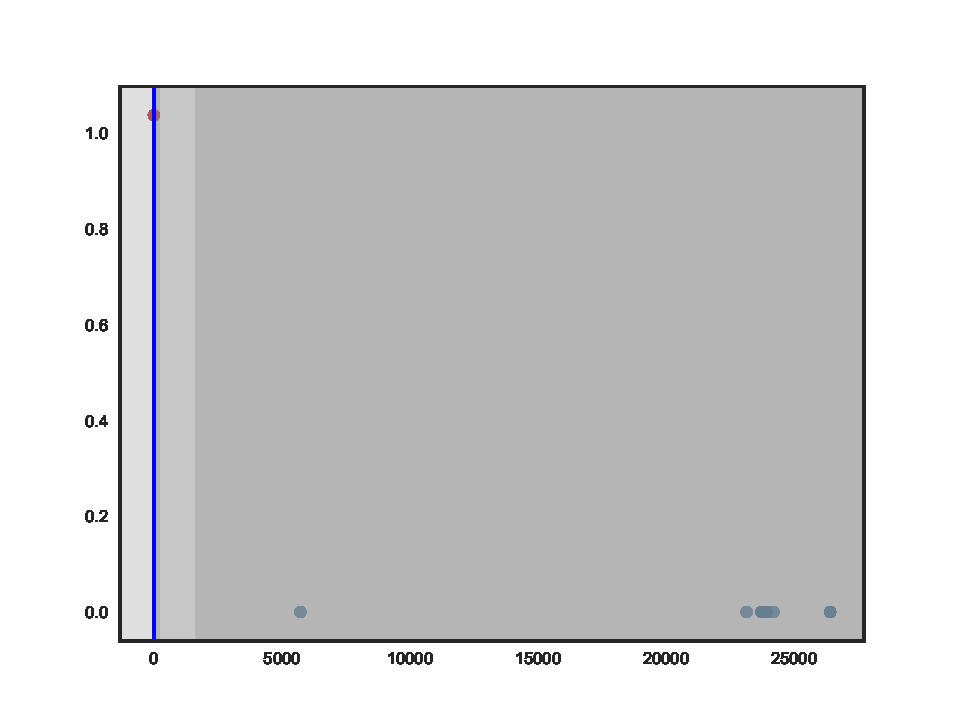
\includegraphics[width=\hsize]{img/toy/unitwise/conv2d_25-2.pdf}} 
    }
    % \hskip1em
    \parbox{.195\textwidth}{%
      \subcaptionbox{Classification layer}{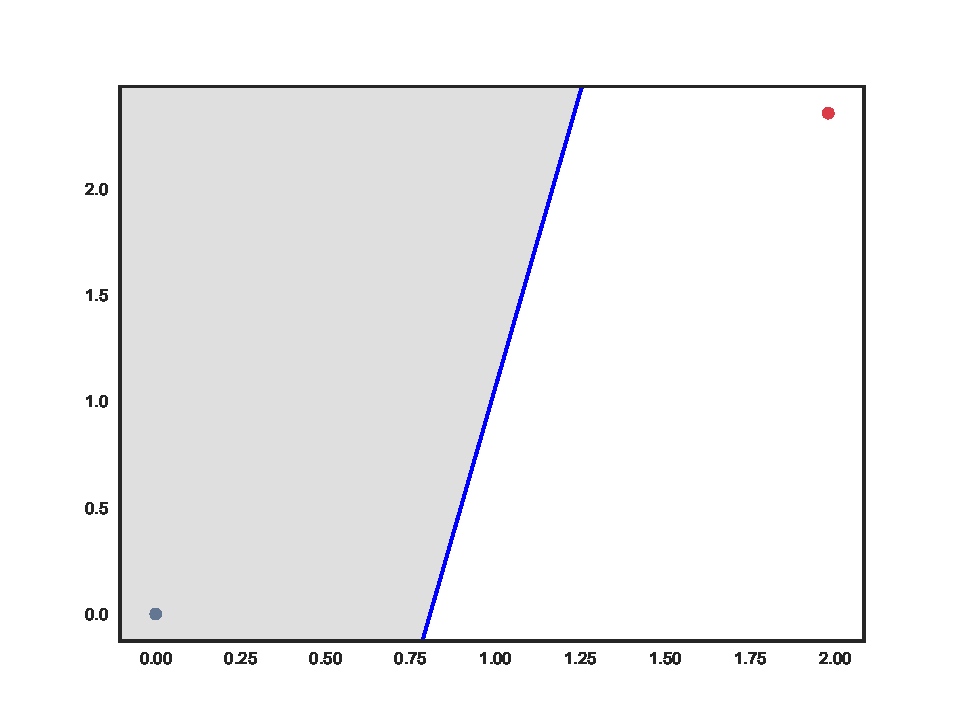
\includegraphics[width=\hsize]{img/toy/unitwise/dense_1-0.pdf}}
    %   \vskip1em
      \subcaptionbox{Classification layer}{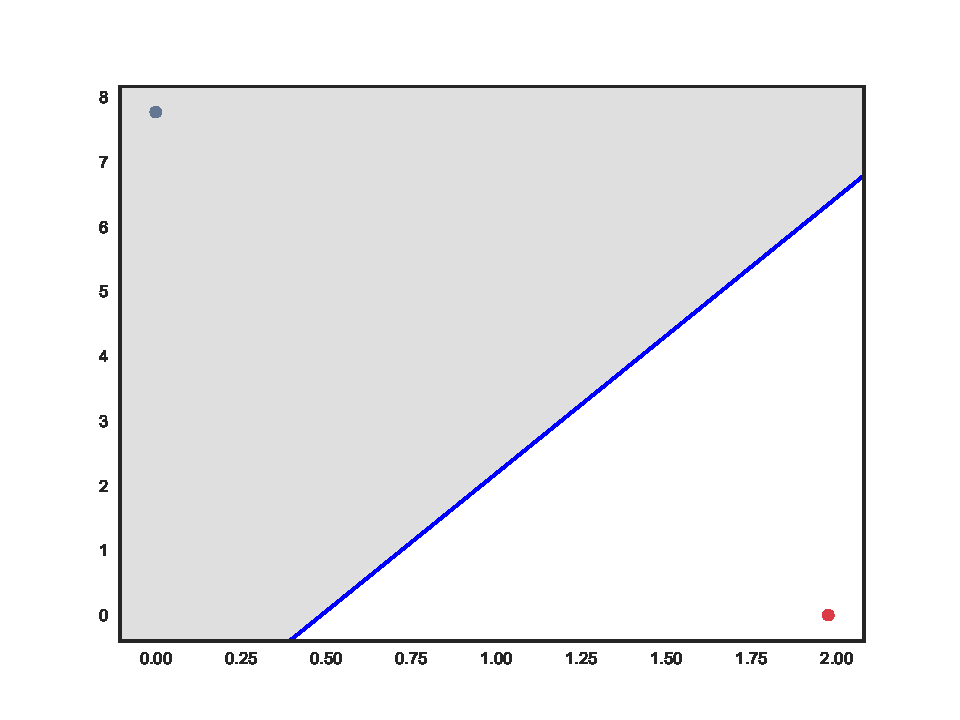
\includegraphics[width=\hsize]{img/toy/unitwise/dense_1-2.pdf}} 
    }
    % \hskip1em
    \parbox{.195\textwidth}{%
      \subcaptionbox{Output}{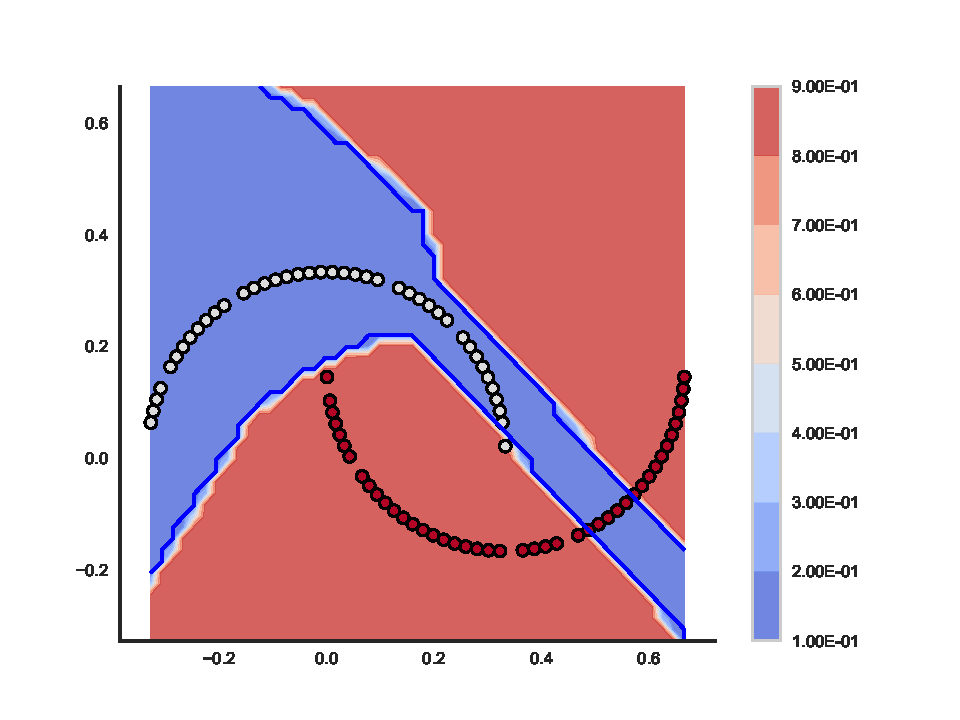
\includegraphics[width=\hsize]{img/toy/unitwise/output.pdf}}
    }
  }
  \caption{\SepUnit}
    \label{fig:moonsUnitwise}
\end{figure*}


Figure \ref{fig:moonsUnitwise} shows our restricted version \SepUnit, which forces all the units of the network to separate but does not consider activation with regard to the points. Because this, solutions like activating all the units of the layer for a single point and sending the rest to zero are still valid. Therefore, we expect it to fail. Notice how even the network fails, the representation found by the network still propagates all way to the input layer and the output is not zero 

\begin{figure*}
  \centering
  %Pointwise
  \parbox{\textwidth}{
    \parbox{.195\textwidth}{%
      \subcaptionbox{Input layer}{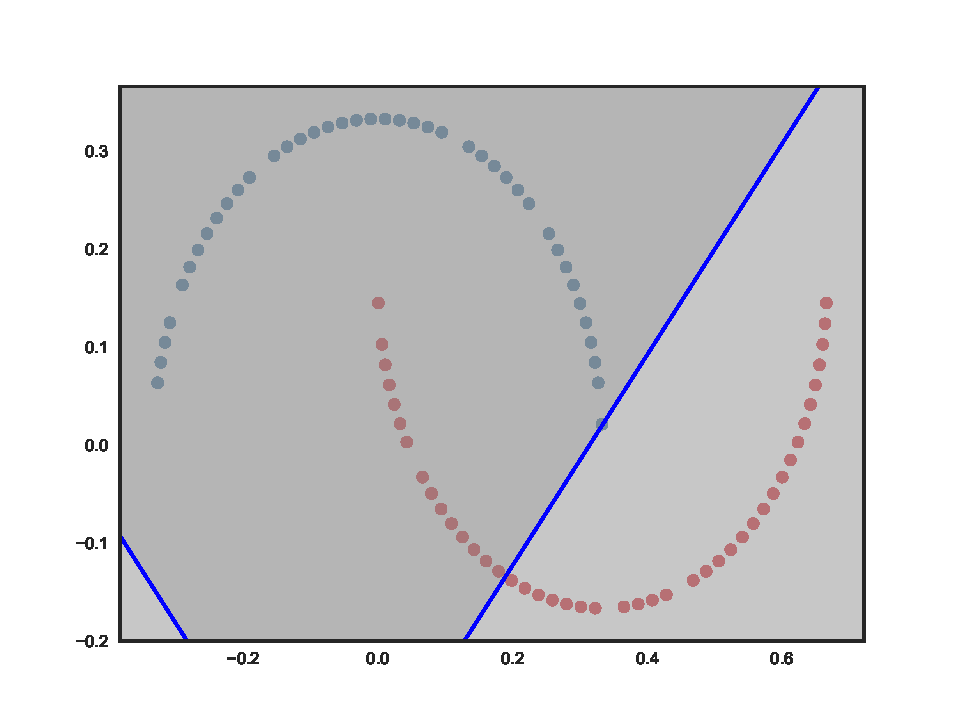
\includegraphics[width=\hsize]{img/toy/pointwise/conv2d_1-0.pdf}}
    }
    % \hskip1em
    \parbox{.195\textwidth}{%
      \subcaptionbox{4th layer}{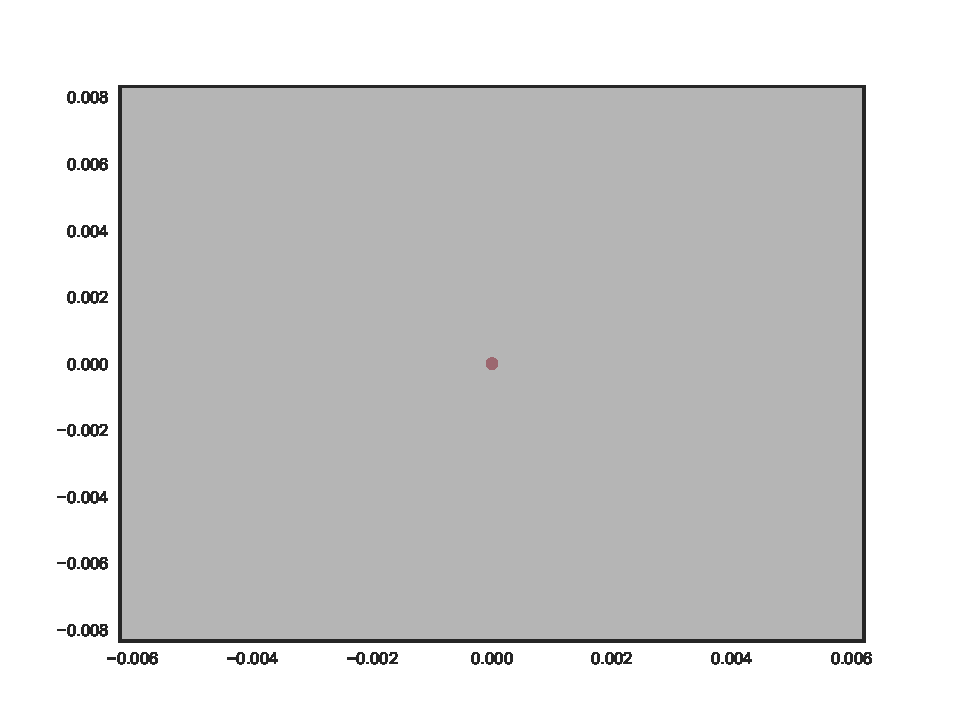
\includegraphics[width=\hsize]{img/toy/pointwise/conv2d_4-0.pdf}}
    %   \vskip1em
      \subcaptionbox{4th layer}{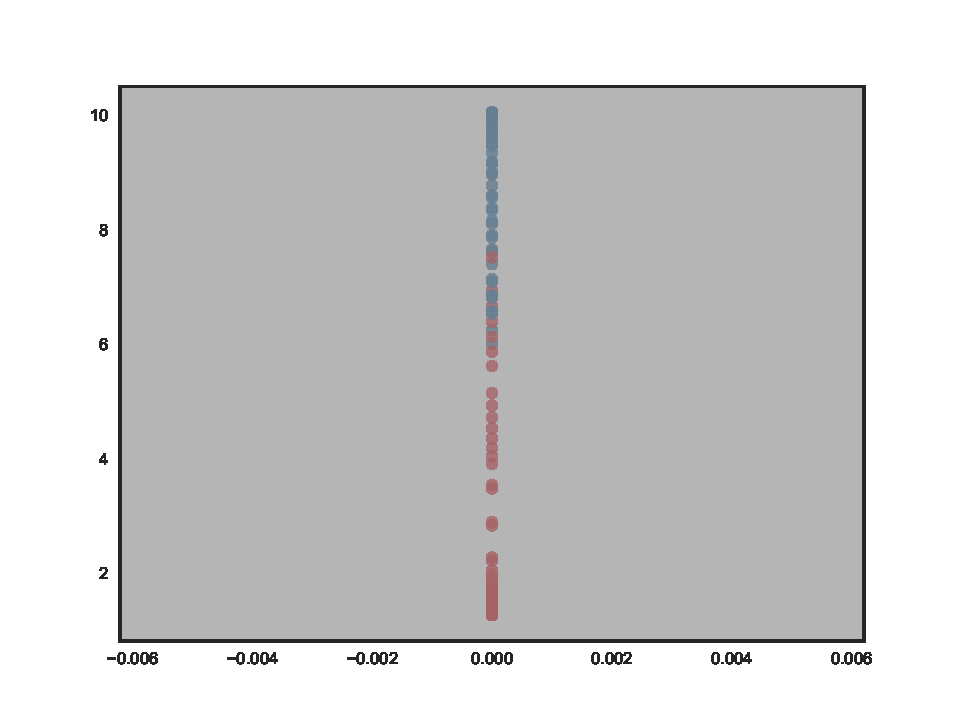
\includegraphics[width=\hsize]{img/toy/pointwise/conv2d_4-2.pdf}} 
    }
    % \hskip1em
    \parbox{.195\textwidth}{%
      \subcaptionbox{25th layer}{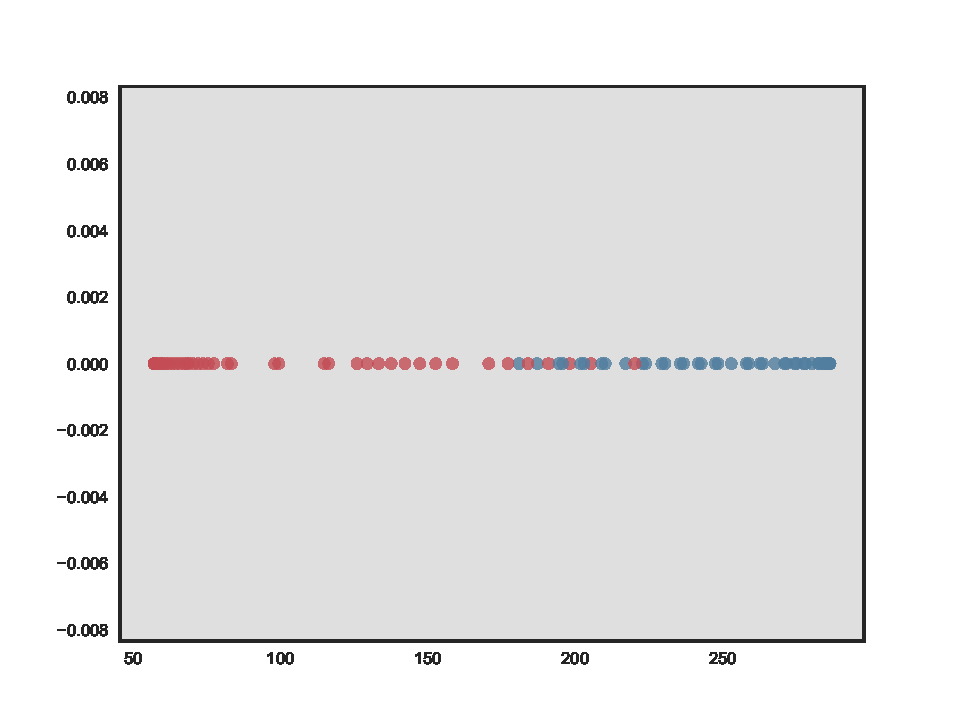
\includegraphics[width=\hsize]{img/toy/pointwise/conv2d_25-0.pdf}}
    %   \vskip1em
      \subcaptionbox{25th layer}{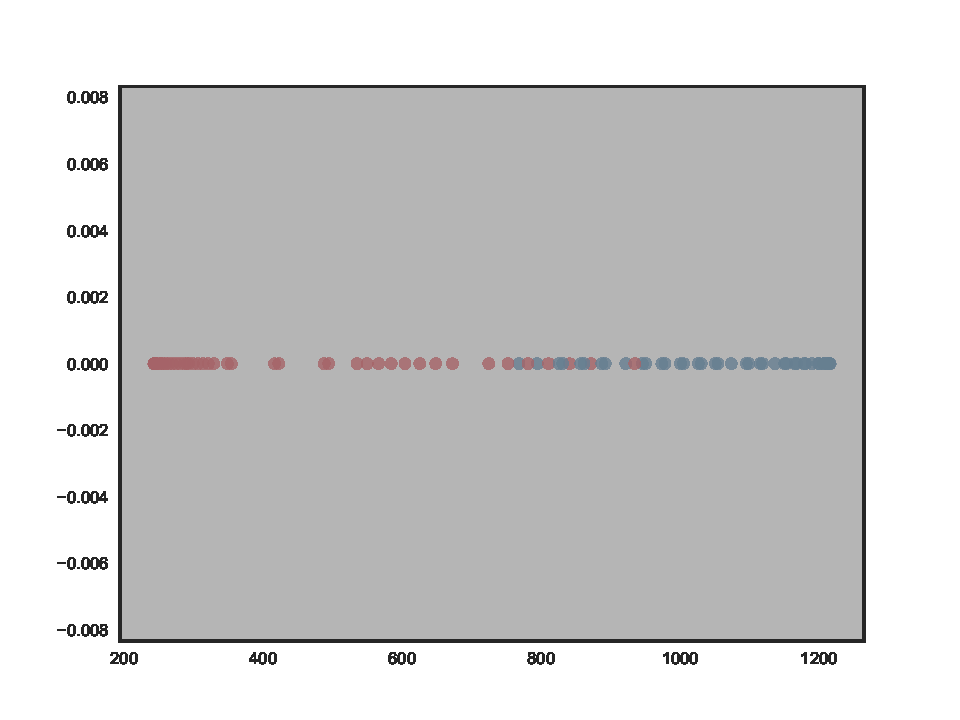
\includegraphics[width=\hsize]{img/toy/pointwise/conv2d_25-2.pdf}} 
    }
    % \hskip1em
    \parbox{.195\textwidth}{%
      \subcaptionbox{}{\includegraphics[width=\hsize]{img/toy/pointwise/dense_1-0.pdf}}
    %   \vskip1em
      \subcaptionbox{}{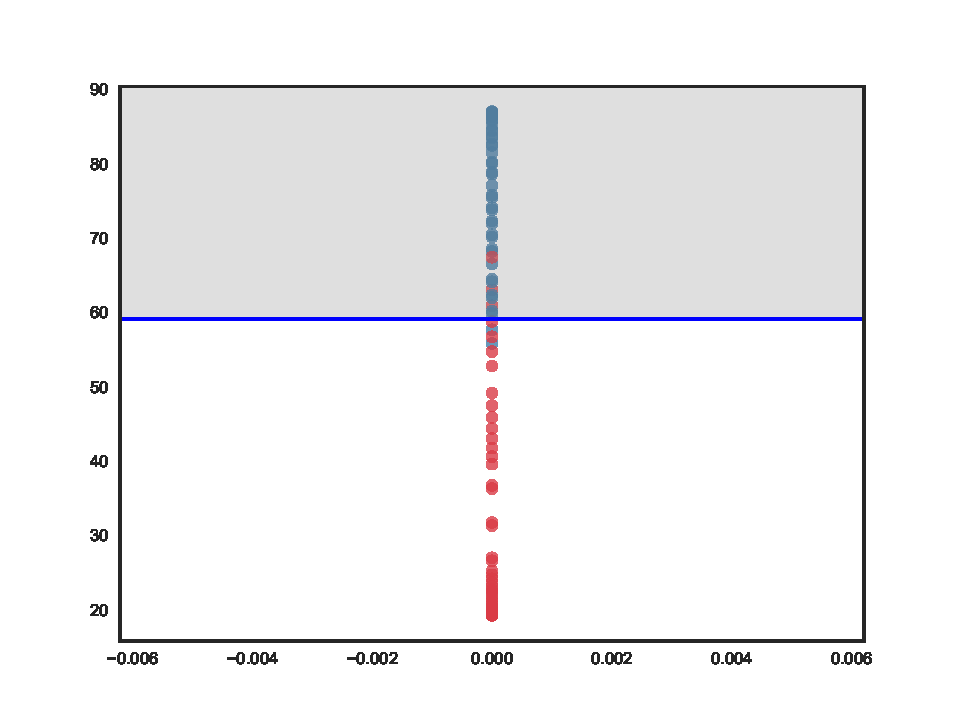
\includegraphics[width=\hsize]{img/toy/pointwise/dense_1-2.pdf}} 
    }
    % \hskip1em
    \parbox{.195\textwidth}{%
      \subcaptionbox{Output}{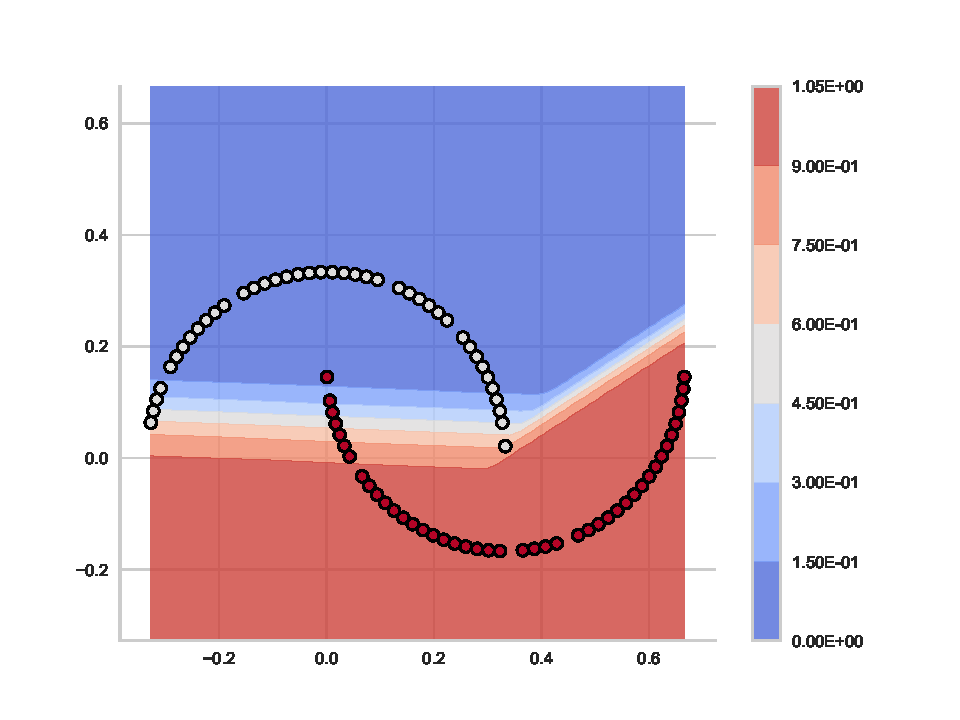
\includegraphics[width=\hsize]{img/toy/pointwise/output.pdf}}
    }
  }
  \caption{\SepPoint}
    \label{fig:moonsPointwise}
\end{figure*}

The constraint \SepPoint is shown at Figure \ref{fig:moonsPointwise}. We see how it effectively propagates the data \emph{topological structure} up to the output of the network ((e), (d), (f), (g)), but as the only requirement that for each point at least one unit is activated and another not this can be fulfilled with an affine unit, so the solution remains almost linear (h). 

\begin{figure*}
  \centering
   \parbox{\textwidth}{
    \parbox{.195\textwidth}{%
      \subcaptionbox{Input layer}{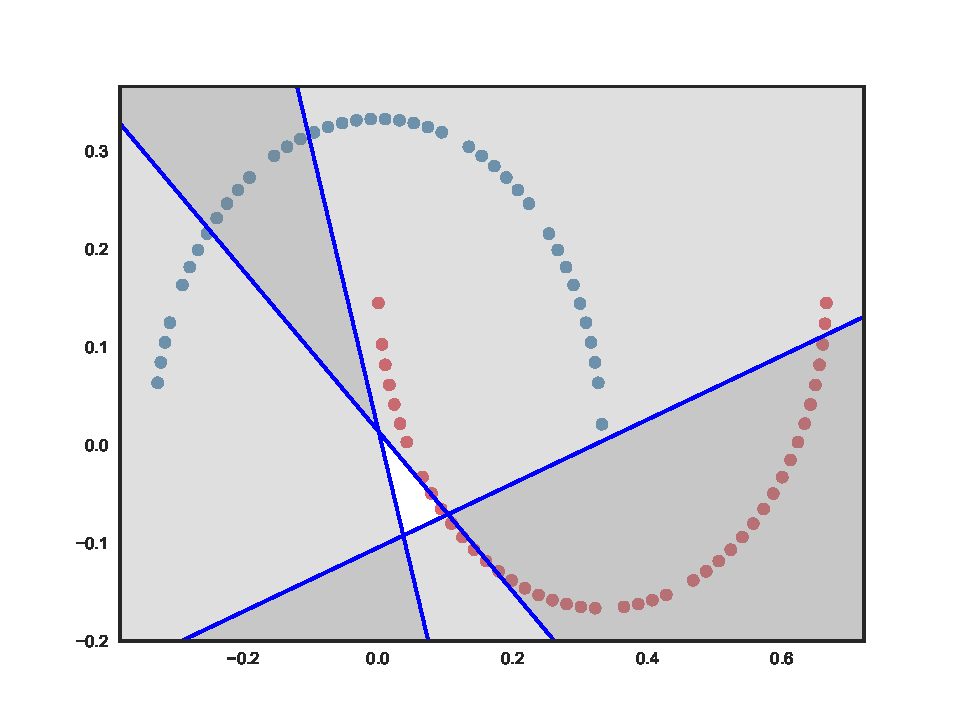
\includegraphics[width=\hsize]{img/toy/unitpointwise/conv2d_1-0.pdf}}
    }
    % \hskip1em
    \parbox{.195\textwidth}{%
      \subcaptionbox{4th layer}{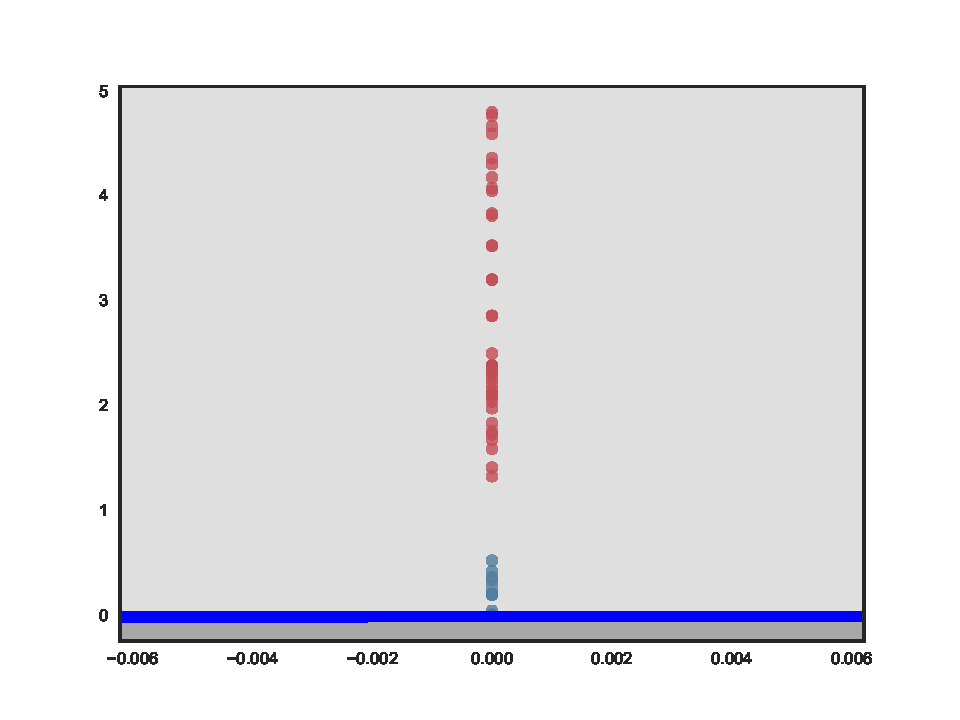
\includegraphics[width=\hsize]{img/toy/unitpointwise/conv2d_4-0.pdf}}
    %   \vskip1em
      \subcaptionbox{4th layer}{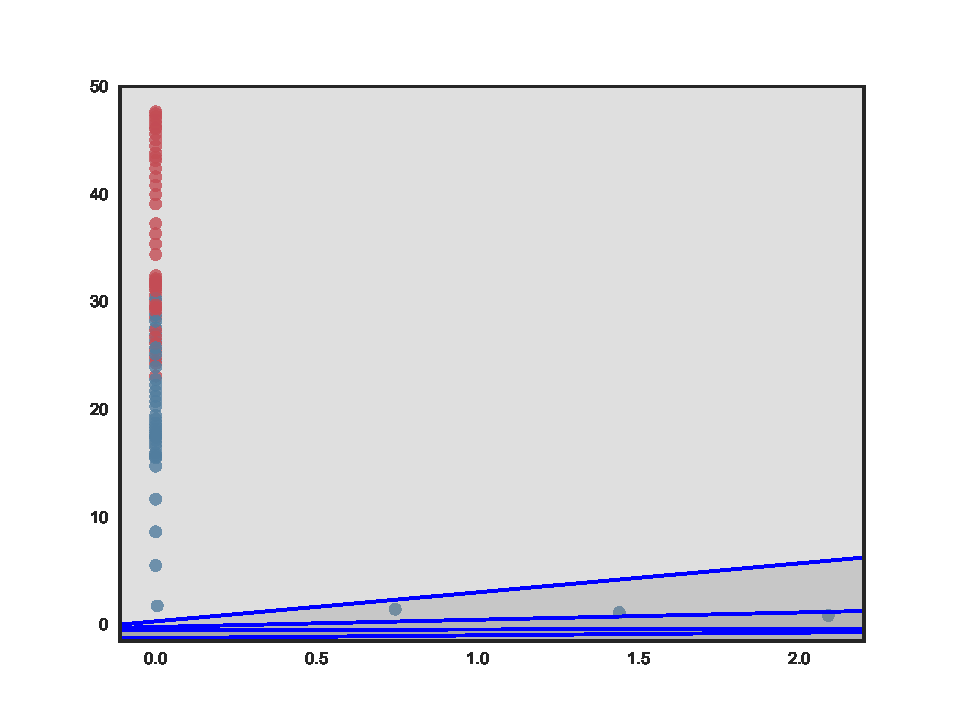
\includegraphics[width=\hsize]{img/toy/unitpointwise/conv2d_4-2.pdf}} 
    }
    % \hskip1em
    \parbox{.195\textwidth}{%
      \subcaptionbox{25th layer}{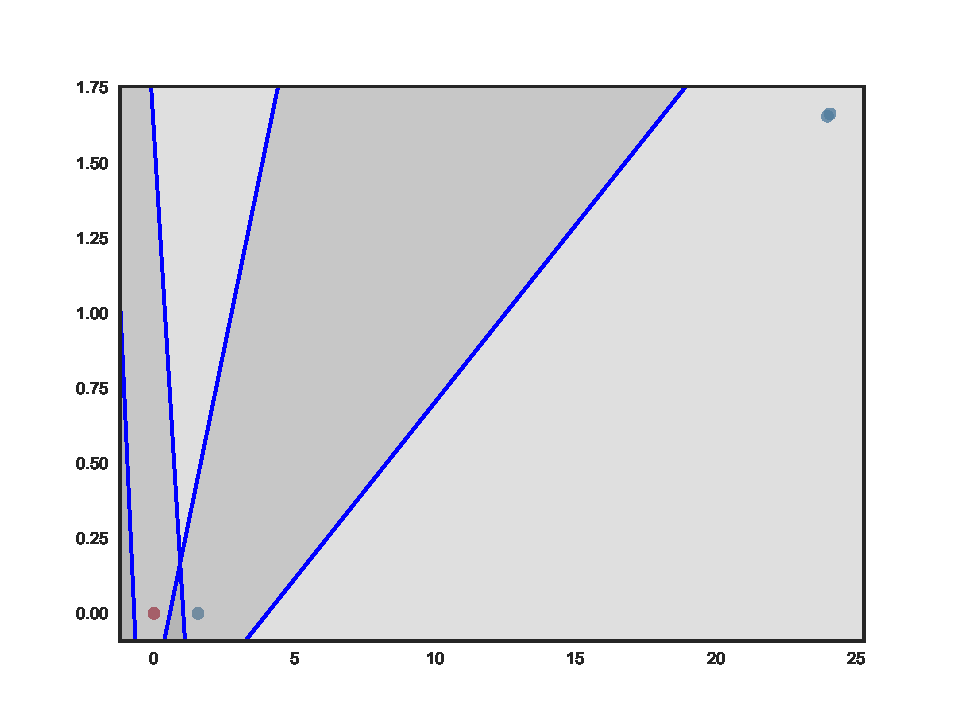
\includegraphics[width=\hsize]{img/toy/unitpointwise/conv2d_25-0.pdf}}
    %   \vskip1em
      \subcaptionbox{25th layer}{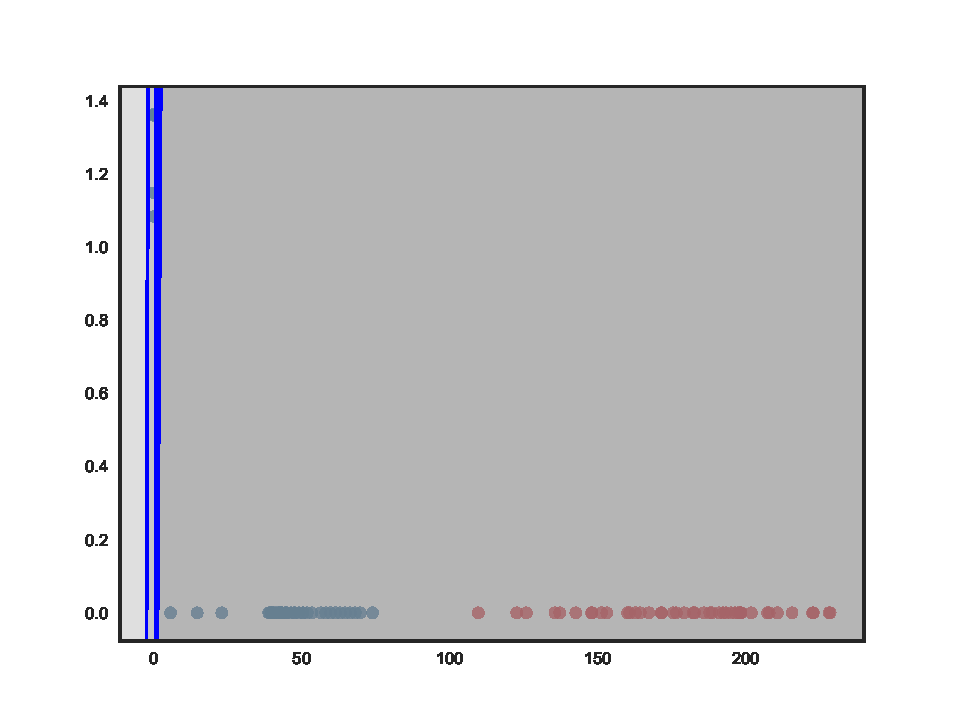
\includegraphics[width=\hsize]{img/toy/unitpointwise/conv2d_25-2.pdf}} 
    }
    % \hskip1em
    \parbox{.195\textwidth}{%
      \subcaptionbox{Classification layer}{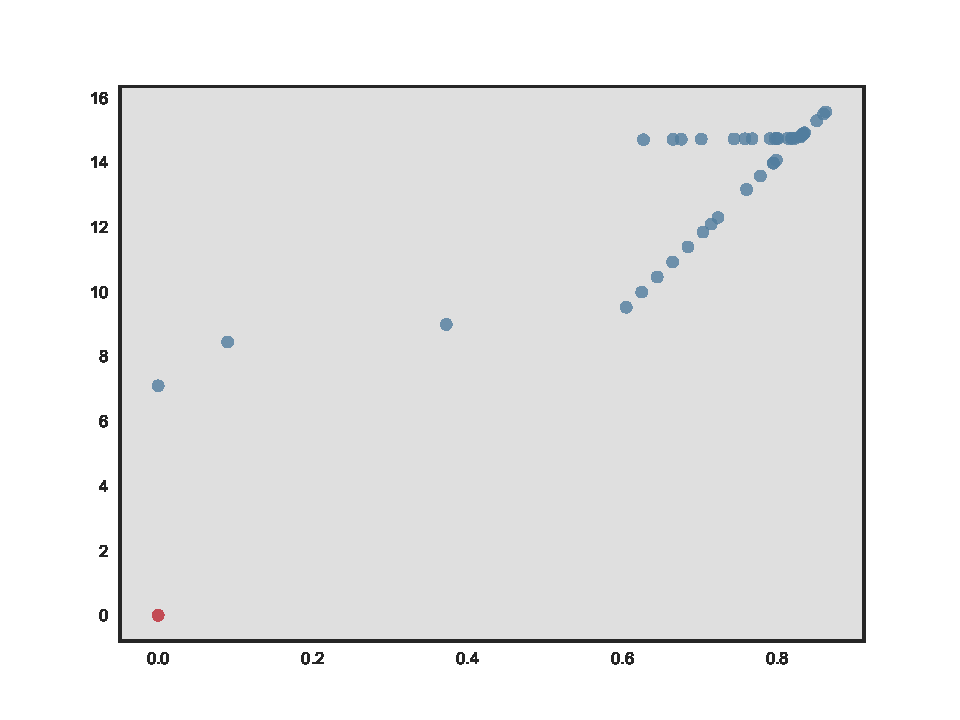
\includegraphics[width=\hsize]{img/toy/unitpointwise/dense_1-0.pdf}}
    %   \vskip1em
      \subcaptionbox{Classification layer}{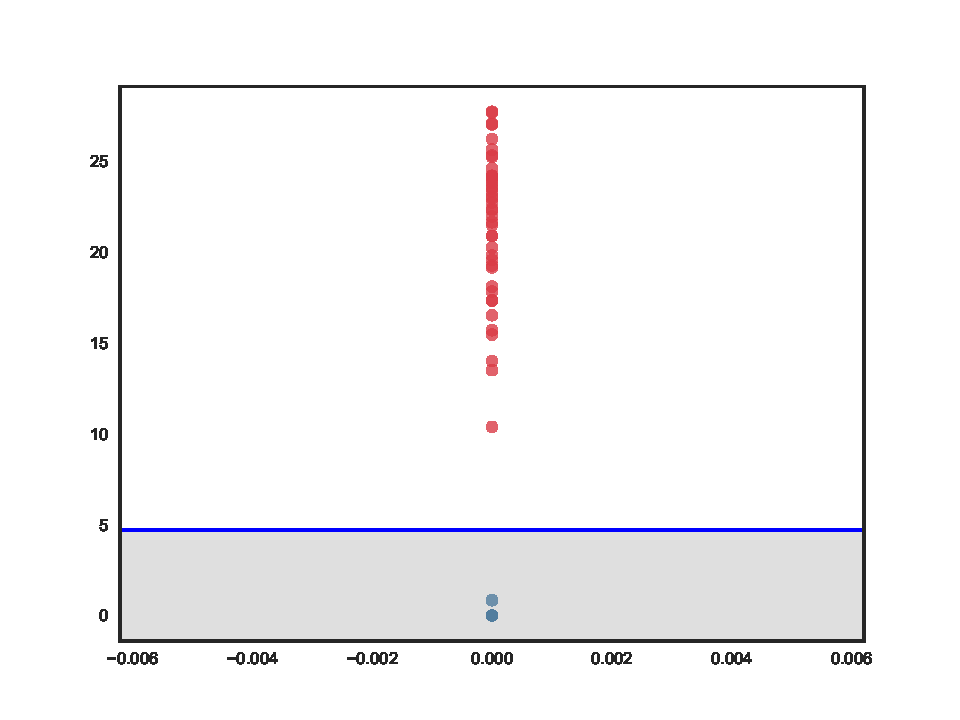
\includegraphics[width=\hsize]{img/toy/unitpointwise/dense_1-2.pdf}} 
    }
    % \hskip1em
    \parbox{.195\textwidth}{%
      \subcaptionbox{Output}{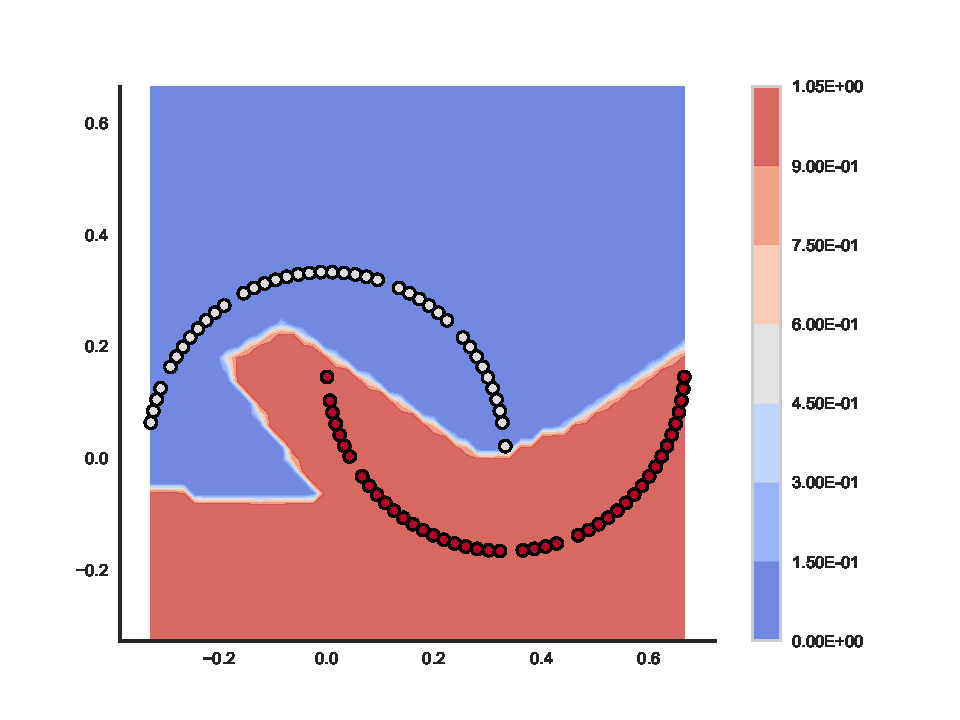
\includegraphics[width=\hsize]{img/toy/unitpointwise/output.pdf}}
    }
  }

    \caption{\SepPointUnit}
    \label{fig:moonsUnitpointwise}
\end{figure*}

Finally, if we combine \SepPoint with \SepPoint in \SepPointUnit, in order to avoid linearity as well as trivial solutions, we find how is effectively separating the data at Figure \ref{fig:moonsUnitpointwise} (h). The solution found is a bit different from \SepLayer at Figure \ref{fig:moonsLayerwise}(h), we due the increased non-linearity of \SepUnit, but thanks to \SepPoint avoids the problems present in Figure \ref{fig:moonsUnitwise}.

\subsection{Separation space}

One interesting question is to understand which effect has the separation constraint by itself, without loss functional. Therefore, we train the same 50x4 network and hyperparameters than the experiment from \ref{subsec:visualization}. Then we leave the network to optimize the different constraints that we propose to see what is the result of enforcing separation and nothing else. We use \ReLU and \ReLUBN for comparison purposes. We show results at Figure \ref{fig:init}.

We find that both \ReLU and \ReLUBN send concentrate all the data  either in a single point in the case of \ReLU and two points in the case of \ReLUBN. It is not surprising their low performance when using them with a loss functional, since it has to spread the points all the way to the input in order to find \emph{useful} representations. In the other hand, we find how \SepLayer connects the output with in the input by sort of linearizing the network, thus outputting something very similar to a linear classifier. This is consistent with \cite{batchnormLinear}, where the authors prove that the network performs best as the units work closest to the linear regime. However, in their work they turn \emph{tanh} activations into lines to find that the depth is increased, whereas we leave the network to decide the units when is better to use a line, to disable itself or perform in a non-linear manner. This effect is also justified due the increase of smoothness across the layers following \cite{haurerandasok}. If we use \SepPointUnit, we see that we lose smoothness but the feature respresentation is still reasonable, showing conectivity among the points, proof that up to some extent topological struture is preserved. Notice how the shape of the input layer is quite similar to the final solution found in Figure \ref{fig:moonsUnitpointwise}(a) when using a loss functional.

\begin{figure*}
  \centering
    \begin{subfigure}[b]{0.3\textwidth}
        \includegraphics[width=\textwidth]{img/init/relu/conv2d_1-0.pdf}
        \caption{\ReLU input layer}
        \label{fig:reluInitInput}
    \end{subfigure}
    ~ %add desired spacing between images, e. g. ~, \quad, \qquad, \hfill etc. 
      %(or a blank line to force the subfigure onto a new line)
    \begin{subfigure}[b]{0.3\textwidth}
        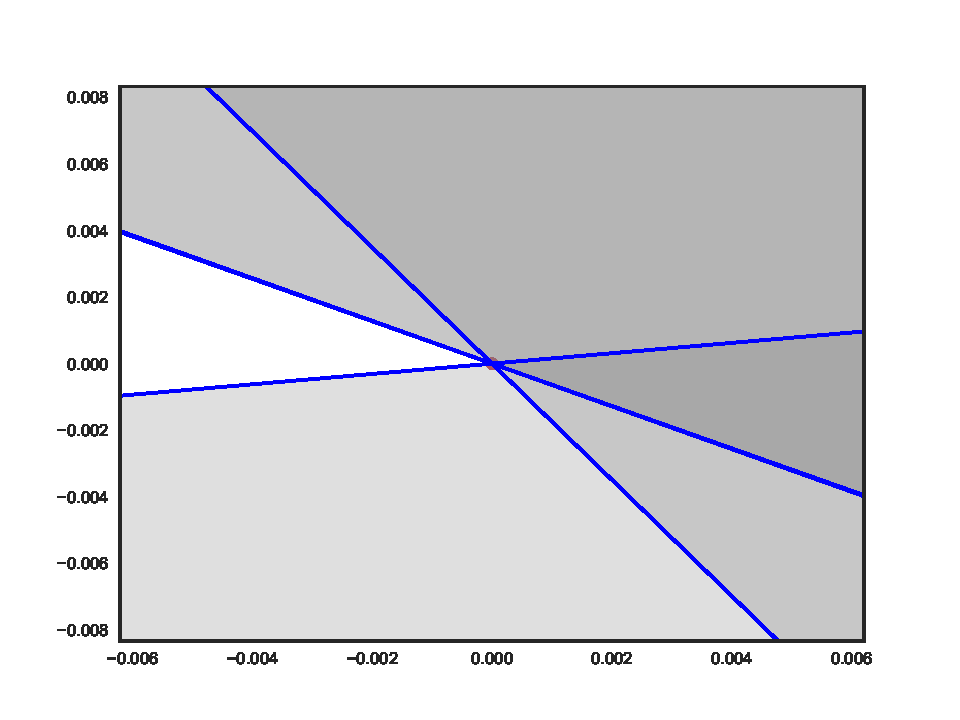
\includegraphics[width=\textwidth]{img/init/relu/conv2d_50-0.pdf}
        \caption{\ReLU 50th layer}
        \label{fig:reluInit501}
    \end{subfigure}
    ~ %add desired spacing between images, e. g. ~, \quad, \qquad, \hfill etc. 
    %(or a blank line to force the subfigure onto a new line)
    \begin{subfigure}[b]{0.3\textwidth}
        \includegraphics[width=\textwidth]{img/init/relu/conv2d_50-2.pdf}
        \caption{\ReLU 50th layer}
        \label{fig:reluIniti502}
    \end{subfigure}
    \\
    \begin{subfigure}[b]{0.3\textwidth}
        \includegraphics[width=\textwidth]{img/init/relu-bn/conv2d_1-0.pdf}
        \caption{\ReLUBN input layer}
        \label{fig:reluBNInitInput}
    \end{subfigure}
    ~ %add desired spacing between images, e. g. ~, \quad, \qquad, \hfill etc. 
      %(or a blank line to force the subfigure onto a new line)
    \begin{subfigure}[b]{0.3\textwidth}
        \includegraphics[width=\textwidth]{img/init/relu-bn/conv2d_50-0.pdf}
        \caption{\ReLUBN 50th layer}
        \label{fig:reluBNInit501}
    \end{subfigure}
    ~ %add desired spacing between images, e. g. ~, \quad, \qquad, \hfill etc. 
    %(or a blank line to force the subfigure onto a new line)
    \begin{subfigure}[b]{0.3\textwidth}
        \includegraphics[width=\textwidth]{img/init/relu-bn/conv2d_50-2.pdf}
        \caption{\ReLUBN 50th layer}
        \label{fig:reluBNInit502}
    \end{subfigure}
    \\
    \begin{subfigure}[b]{0.3\textwidth}
        \includegraphics[width=\textwidth]{img/init/layerwise/conv2d_1-0.pdf}
        \caption{\SepLayer input layer}
        \label{fig:layerwiseInitInput}
    \end{subfigure}
    ~ %add desired spacing between images, e. g. ~, \quad, \qquad, \hfill etc. 
      %(or a blank line to force the subfigure onto a new line)
    \begin{subfigure}[b]{0.3\textwidth}
        \includegraphics[width=\textwidth]{img/init/layerwise/conv2d_50-0.pdf}
        \caption{\SepLayer 50th layer}
        \label{fig:layerwiseInit501}
    \end{subfigure}
    ~ %add desired spacing between images, e. g. ~, \quad, \qquad, \hfill etc. 
    %(or a blank line to force the subfigure onto a new line)
    \begin{subfigure}[b]{0.3\textwidth}
        \includegraphics[width=\textwidth]{img/init/layerwise/conv2d_50-2.pdf}
        \caption{\SepLayer 50th layer}
        \label{fig:layerwiseInit502}
    \end{subfigure}
    \\
    \begin{subfigure}[b]{0.3\textwidth}
        \includegraphics[width=\textwidth]{img/init/unitpointwise/conv2d_1-0.pdf}
        \caption{\SepPointUnit Input}
        \label{fig:unitpointInitInput}
    \end{subfigure}
    ~ %add desired spacing between images, e. g. ~, \quad, \qquad, \hfill etc. 
      %(or a blank line to force the subfigure onto a new line)
    \begin{subfigure}[b]{0.3\textwidth}
        \includegraphics[width=\textwidth]{img/init/unitpointwise/conv2d_50-0.pdf}
        \caption{\SepPointUnit 50th layer}
        \label{fig:unitpointInit501}
    \end{subfigure}
    ~ %add desired spacing between images, e. g. ~, \quad, \qquad, \hfill etc. 
    %(or a blank line to force the subfigure onto a new line)
    \begin{subfigure}[b]{0.3\textwidth}
        \includegraphics[width=\textwidth]{img/init/unitpointwise/conv2d_50-2.pdf}
        \caption{\SepPointUnit 50th layer}
        \label{fig:unitpointInit5012}
    \end{subfigure}
    
  \caption{This figure shows the input and feature layers of network composed of 50 layers of 4 units each. The network is trained without loss, implying that for \ReLU it is left as it was initialized and in the case of \ReLUBN $10000$ epochs are run in order to ensure that the moments are adjusted. We train also \SepLayer until convergence in order to understand what changes are undergoing in the network if we only optimize the separation constraint, without additional loss. We find that the Glorot initialization used with \ReLU is quite poor with regards to the resulting representation in the feature layer, as we see in ((b), (c)). As we see in \ref{fig:moonsReLU}, \ReLU tends to pack all the data to zero as the network grows in depth, disregarding the initialization. \ReLUBN is able to push some data from zero, see (d), but still packs all the data in two points ((e, (f)). This leads to the fact that the input layer remains the same than \ReLU's, see (a) and (d). If we look at \SepLayer (h) and (i), we see how the feature space is much more linear and how topological structure is somewhat preserved, which is easy to understand when one sees the plane placement in the input layer (g). Finally, \SepPointUnit shows a much more non-linear representation at (k) and (l), although the separation is much more unintuitive.} 
  \label{fig:init} 
\end{figure*}

% \begin{figure*} 
%     \centering
%   \subfloat[\ReLU input \label{fig:reluInputInit}]{%
%       \includegraphics[width=0.20\linewidth]{img/init/relu/0.pdf}}
%   \subfloat[\ReLU feature layer \label{fig:reluInputFeatureInit}]{%
%         \includegraphics[width=0.20\linewidth]{img/init/relu/49.pdf}}
%   \subfloat[\ReLUBN input at epoch 40 \label{fig:relubnInputInit}]{%
%         \includegraphics[width=0.20\linewidth]{img/init/relu-bn/0.pdf}}
%   \subfloat[\ReLUBN feature layer at epoch 40 \label{fig:relubnFeatureInit}]{%
%       \includegraphics[width=0.20\linewidth]{img/init/relu-bn/48.pdf}}
%       \\
%   \subfloat[\SepLayer input at epoch 0 \label{fig:sepInitInput0}]{%
%       \includegraphics[width=0.20\linewidth]{img/init/layerwise/0/0.pdf}}
%   \subfloat[\SepLayer feature layer at epoch 0 \label{fig:sepInitFeature0}]{%
%         \includegraphics[width=0.20\linewidth]{img/init/layerwise/0/49.pdf}}
%   \subfloat[\SepLayer input at epoch 16 \label{fig:sepInitInput16}]{%
%       \includegraphics[width=0.20\linewidth]{img/init/layerwise/16/0.pdf}}
%   \subfloat[\SepLayer feature layer at epoch 16 \label{fig:sepInitInput16}]{%
%         \includegraphics[width=0.20\linewidth]{img/init/layerwise/16/49.pdf}}
%         \\
%   \subfloat[\SepLayer input at epoch 32\label{fig:sepInputInit32}]{%
%       \includegraphics[width=0.20\linewidth]{img/init/layerwise/32/0.pdf}}
%   \subfloat[\SepLayer feature layer at epoch 32\label{fig:sepInputInit32}]{%
%         \includegraphics[width=0.20\linewidth]{img/init/layerwise/32/49.pdf}}
% \subfloat[\SepLayer input at epoch 48\label{fig:sepInputInit48}]{%
%       \includegraphics[width=0.20\linewidth]{img/init/layerwise/48/0.pdf}}
%   \subfloat[\SepLayer feature layer at epoch 48 \label{fig:sepInputInit48}]{%
%         \includegraphics[width=0.20\linewidth]{img/init/layerwise/48/49.pdf}}

%   \caption{This figure shows the input and feature layers of network composed of 50 layers of 4 units each. The network is trained without loss, implying that for \ReLU it is left as it was initialized and in the case of \ReLUBN a number of epochs is run in order to ensure that the moments are adjusted. We train also \SepLayer for a number of epochs in order to understand what changes are undergoing in the network if we only optimize the separation constraint, without no additional loss. We find that the Glorot initialization used with \ReLU is quite poor with regards to the resulting representation in the feature layer, as we see in (b). As we see in \ref{fig:toy}, \ReLU tends to pack all the data to zero as the network grows in depth, disregarding the initialization. \ReLUBN is able to push some data from zero, see (d), but we argue that this is product of the biases of the network, other than a real connection with the data. This leads to the fact that the input layer remains the same than \ReLU's, see (c). If we look at \SepLayer (e-l), we see how at the beginning ((e), (f)) the starting point is indeed the same than \ReLU, but incrementally thanks to the separating constraint, it pushes the hyperplanes all the way back to the input (g) so it is able to have a much better representation at (j).} 
%   \label{fig:init} 
% \end{figure*}

\subsection{Results concerning Accuracy}\label{subsec:accuracyResults}
To gauge accuracy between \ReLU, \ReLU +  batchnorm (\texttt{\ReLU+BN}), and \SepUnit we tested all variants of \SepUnit as described on definition \ref{def:separationConstraints} for the \moons dataset, introducing also  \SepPointUnit combining \SepUnit and \SepPoint. \SepUnit shows a disparity in improvements against batchnorm, between both datasets, but shows significant improvements over the basic \ReLU baseline (that yields \emph{trivial} accuracies of $40$\% in \moons and $10$\% in \cifar), under the Glorot initialization scheme. The reader can observe Table \ref{tab:moons} for \moons (where all \SepConstraint variants were tested) and Table \ref{tab:cifar10} for \cifar (displaying only \SepLayer) for verification. 
\\\\
In the \moons dataset constraint introductions demonstrate \emph{perfect} accuracy, whereas batchnorm falls behind to $60$\%.  In contrast maximal \cifar accuracy yielded a $56.82$\% using \SepLayer, against a $56.03$\% maximal accuracy of batchnorm. In matters of the differences between the variants of the constraints, testing done with the \moons dataset (as presented in Table \ref{tab:scopes}, \SepLayer achieves maximal accuracy in the \moons dataset.  When combining batchnorm and constraints (of \SepLayer type) a maximal accuracy of $58.80$\% is reached using batch sizes of $64$ and $128$.  
\\\\
When considering \emph{overfitting}, \SepLayer shows a reduction in overfitting in contrast to \ReLUBN (20\% in \moons and 30\% for \cifar), while \SepLayer shows a drop of $3\%$ in \cifar and $0$\%. When changing the initialization scheme to zero in \cifar using \SepLayer we observe that accuracy increases to $58.12$\%. \ReLUBN and \ReLU \emph{cannot} function using zero initialization. In addition, Figure \ref{fig:ZeroVsGlorotDifference} displays the gaps between train and validation accuracy for the \cifar dataset as a histogram (over 44 runs, discarding experiments with accuracies lower than $30$\%), while Figure \ref{fig:zeroConvergence}, shows that zero initialization delays the exploding gradient breakdown in accuracy, a phenomenon that is observed using the highest learning rate for \cifar, $\gamma=0.001$. 
\begin{table}[h!]
\begin{center}
\begin{tabular}{l|rr|rr}
\toprule
{}  & \multicolumn{2}{c}{Accuracy} & \multicolumn{2}{c}{Loss} \\
{}  & Train   & Val.  & Train  & Val.  \\
\midrule
\ReLU            &  0.5176 &      0.4 &  0.6925 &  0.6938 \\
\ReLUBN     &  0.8117 &      0.6 &  0.6331 &  0.6636 \\
\SepUnit &  1.0000 &      1.0 &  0.0000 &  0.0211 \\
\bottomrule
\end{tabular}
\end{center}
\caption{Maximal performance results for the toy experiment using the \moons dataset. From left to right, accuracy and loss (for \emph{train} and \emph{validation} sets) for \ReLU, \ReLUBN, and  \SepUnit in all its variants.}
  \label{tab:moons}
\end{table}

\begin{table}[h!]
\begin{center}
\begin{tabular}{l|rr|rr}
\toprule
{}  & \multicolumn{2}{c}{Accuracy} & \multicolumn{2}{c}{Loss} \\
{}  & Train   & Val.  & Train  & Val.  \\
\midrule
\ReLU              &  0.0970 &   0.1000 &  2.3025 &  2.3025 \\
\ReLUBN            &  0.8300 &   0.5603 &  0.4614 &  1.2391 \\
\SepUnit*    &  0.6172 &   0.5812 &  1.0665 &  1.1867 \\
\bottomrule
\end{tabular}
\end{center}
\caption{Maximal performance results for the \cifar dataset. From left to right, accuracy and loss (for \emph{train} and \emph{validation} sets) for \ReLU, \ReLUBN, and  \SepUnit in all its variants. (*) Zero initialization for \SepUnit was used. }
  \label{tab:cifar10}
\end{table}

\begin{table}[h]
\begin{center}
\begin{tabular}{l|rr|rr}
\toprule
{}  & \multicolumn{2}{c}{Accuracy} & \multicolumn{2}{c}{Loss} \\
{}  & Train   & Val.  & Train  & Val.  \\
\midrule
\SepLayer    &  1.0000 &  1.0000 &  0.0000 &  0.0211 \\
\SepPoint    &  0.9294 &  0.8000 &  0.1765 &  0.6476 \\
\SepUnit    &  0.9058 &  0.8000 &  0.4161 &  1.5228 \\
\SepPointUnit   &  0.9882 &  0.9333 &  0.6988 &  1.0810 \\
\bottomrule
\end{tabular}
\end{center}
\caption{Comparison between maximal performances of all \SepUnit variants using \moons dataset. From left to right, accuracy, and loss are presented (for \emph{train} and \emph{validation} sets).}
  \label{tab:scopes}
\end{table}


\begin{table}[h]
\begin{center}
\begin{tabular}{l|rr|rr}
\toprule
{}  & \multicolumn{2}{c}{Accuracy} & \multicolumn{2}{c}{Loss} \\
{}  & Train   & Val.  & Train  & Val.  \\
\midrule
Glorot &  0.6739 &   0.5682 &  0.9114 &  1.2673 \\
Zeros  &  0.6172 &   0.5812 &  1.0665 &  1.1867 \\
\bottomrule
\end{tabular}
\end{center}
\caption{Maximal performance comparison between initialization schemes using the \cifar dataset. From left to right, accuracy and loss (for \emph{train} and \emph{validation} sets) for Glorot and Zeros initializations.}
  \label{tab:zero_cifar}
\end{table}


\begin{table}[h]
\begin{center}
\begin{tabular}{l|rr|rr}
\toprule
{}  & \multicolumn{2}{c}{Accuracy} & \multicolumn{2}{c}{Loss} \\
{}  & Train   & Val.  & Train  & Val.  \\
\midrule
\ReLUBN           &  0.8300 &   0.5603 &  0.4614 &  1.2391 \\
\SepUnit    &  0.6739 &   0.5682 &  0.9114 &  1.2673 \\
\SepLayerBN&  0.84758 &   0.5880 &  0.4128 &  1.2095 \\
\bottomrule
\end{tabular}
\end{center}

\caption{Maximal performance results for the \cifar dataset. From left to right, accuracy and loss (for \emph{train} and \emph{validation} sets) for \ReLUBN,  \SepLayer, and \SepLayerBN}
\label{tab:sc-relu-bn}
\end{table}

\subsection{The Effect of Constraint Loss}\label{subsec:constraintLoss}
The constraint loss \ref{eq:constraintloss}, measures the  violation of the constraints \cite{florenzano2001ConvexAnalysis,Burges1998TutorialOnSVMForPatternRecognition}, besides the obvious relation between loss and accuracy \cite{LeCun06atutorial,lecun2015DeepLearningBig}, for the case of \SepUnit, we must notice that the total Loss of training a DNN with \SepUnit (equation \ref{eq:constraintLossFunctional}) linearly combines cross-entropy loss and constraint loss, that constructs a training sequence composed of two gradients, that yields a non-linear combination of the learning rate $\gamma$ and the constraint loss parameter $\lambda$ (a substitution into equation \ref{eq:trainingSequence}), so that the resulting training sequence is of the form.
\begin{equation}\label{eq:resultingConstraintLoss}
\theta_{n+1} = \theta_n - \gamma\nabla_{\theta}\mathcal{L}-\sum_{\xi\in\Xi}\lambda\gamma\nabla\xi.
\end{equation}
Choosing the zero initialization scheme implies choosing $\theta_0=\vec{0}$ or otherwise on the Glorot scheme. As Figure \ref{fig:peaks} showcases, variations in $\xi$ (i.e. constraint loss) have a direct impact on accuracy.  From a geometric point of view, the values of $\xi$ aim to ensure that zero sets of layers are non-empty in their intersection with the training set (a consequence of the topological fact in remark \ref{remark:topologicalFacts}): choosing Glorot initialization (and in a worse case the zero initialization) may yield a violation of both constraints and remark \ref{remark:topologicalFacts} starting the total loss at an arbitrary high value (in Figure \ref{fig:peaks} reaching a value of $79$ in the first epochs).     
\\\\
In addition, Figure \ref{fig:peaks} also showcases the relation between values of the constraint loss in relation to validation accuracy that are significant. After drops in constraint loss, accuracy changes abruptly (see the behavior around iteration 458, where accuracy drops to 21\%), such conclusion is reached also when observing Figures \ref{fig:lambdas} and \ref{fig:constraintLoss} (in the case of \cifar). Increasing values of $\lambda$ reinforces the positive effect that constraint loss has on cross-entropy, and even more so in the presence of zero initialization. However, constraint loss cannot be the sole factor in accuracy increases (notice the abrupt increase in accuracy around iteration $750$). We observe that cross-entropy loss has a much direct impact in overall accuracy, as presented by Figure \ref{fig:peaks}: around iteration $750$, the cross-entropy loss suffers an abrupt change, that increases accuracy until iteration $1750$.   
\\\\
In matters of the influence of Glorot and zero initialization, Figure \ref{fig:zeroConvergence} shows that lower values of $\gamma$ ensure convergence in accuracy. Zero initialization allows the training sequence to reach a higher value (as noted in subsection \ref{subsec:accuracyResults}), but also in less epochs. However, Glorot initialization yields a an almost monotonic behavior of accuracy, in contrast to the \emph{oscillating} behavior observed using both schemes, as parts \ref{fig:glorotWeightGradient} and \ref{fig:zerosWeightGradient} of Figure \ref{fig:histo} suggest. We must recall that the geometric formulation underlying \SepUnit merely guarantees non-empty zero sets and non-empty supports. However, this oscillatory dynamic could constitute evidence of \emph{data shattering} \cite{Zhang2016RethinkingGeneralization}. Still, the role of the \emph{balance} parameter \ref{eq:separatingUnit} which is needed to bias the constraint to the positive side in order to break symmetry requires more research.
\\\\
Upon closer look, the histograms for weights and bias presented in Figure \ref{fig:histo}, suggest that Glorot may lead to data shattering (choosing more \emph{disperse} weights throughout training, as presented in part \ref{fig:glorotWeights}), while the variance of weights under the zero initialization is lower (part \ref{fig:zerosWeights}). From a geometric point of view, the zero initialization leads to \emph{smaller} normal vectors for separating planes. However, as Figures \ref{fig:glorotBias} and \ref{fig:zerosBias} showcase, possible bias  compose a wide range in both initialization schemes: $[-0.6,0.2]$ for Glorot, while its range is $[-0.02,0.18]$. This could contradict the fact that separation \emph{must occur} on the first orthant $\Real{4}$, however without correlations between weights and bias, such conclusion cannot be reached beyond intuition.    
\\\\
From a geometric stand point, this oscillating phenomena has a very intuitive explanation. As points are mapped through the intermediate representations, they sometimes fall into zero set of a layer, while weights and biases are being updated, moving in between zero set and support that are divided via the hyperplane described in equation \ref{eq:supportAndZerosOfUnit}. From the point of view of hyperplanes, this amounts to swapping the signs of normal vectors, sometimes in harmony with the bias, sometimes against it (see iterations 500 to 600 in Figure \ref{fig:peaks}). 
\\\\
In matters of implementation, the two parts of the predicates in the constraint formulation are involved (recall equations \ref{eq:constraintLinearFormulation} and \ref{eq:predicateForSepUnitP}) for the maximum and minimum values of $p$. These induce two constraints, that are void under the zero initialization.  In order to break the tie, we use a convex combination of both constraints biasing them at $0.51$ (towards the side of maximum). So that this small bias \emph{jumpstarts} the network into action.  

\begin{figure}[h]
  \centering  
	\includegraphics[width=0.5\textwidth]{constraint_loss}
      \caption{Scatter plot of constraint loss versus accuracy involving all successful tests with \cifar.}
\label{fig:constraintLoss}
\end{figure}

\begin{figure}[h]
\centering    
\includegraphics[width=0.5\textwidth]{lambdas}
      \caption{Accuracy versus $\lambda$. Left-hand side using Glorot initialization scheme. Right-hand side using zero intialization scheme.}
\label{fig:lambdas}
\end{figure}

\begin{figure*}[h]
  \begin{center}
    \includegraphics[width=1.0\textwidth]{peaks}
      \caption{Evolution of training throughout epochs (cross-entropy, constraint loss, and accuracy). Left-hand axis show the accuracy metric (blue line) against the cross-entropy, and constraint loss in the right axis (orange line), for each epoch of the training phase in the horizontal axis.}
			\label{fig:peaks}
\end{center}
\end{figure*}

\begin{figure*}[h]
  \centering
		\includegraphics[width=1.0\textwidth]{zeros-vs-glorot}
      \caption{Convergence plot for the evolution of the validation accuracy during the training phase. Solid lines stand for Zero initialization, dashed stand for Glorot initialization. The colors encode the different learning rates $\gamma$ used, red for $0.001$, green for $0.0005$ and blue for $0.0001$.}
\label{fig:zeroConvergence}
\end{figure*}

\begin{figure}[h!]
\centering
    \includegraphics[width=0.5\textwidth]{zeros-vs-glorot-val-difference}
      \caption{Histogram of gaps between train and validation accuracy, for Zero and Glorot initialization over all successful runs of \cifar.}
		\label{fig:ZeroVsGlorotDifference}


\end{figure}

\begin{figure} 
    \centering
  \subfloat[Glorot weights\label{fig:glorotWeights}]{%
       \includegraphics[width=0.45\linewidth]{glorot-kernel.png}}
    \hfill
  \subfloat[Zeros weights\label{fig:zerosWeights}]{%
        \includegraphics[width=0.45\linewidth]{zeros-kernel.png}}
    \\
  \subfloat[Glorot weight gradient\label{fig:glorotWeightGradient}]{%
        \includegraphics[width=0.45\linewidth]{glorot-kernel-grad.png}}
    \hfill
  \subfloat[Zeros weight gradient\label{fig:zerosWeightGradient}]{%
        \includegraphics[width=0.45\linewidth]{zeros-kernel-grad.png}}
        
   \subfloat[Glorot bias\label{fig:glorotBias}]{%
       \includegraphics[width=0.45\linewidth]{glorot-bias.png}}
    \hfill
  \subfloat[Zeros bias\label{fig:zerosBias}]{%
        \includegraphics[width=0.45\linewidth]{zeros-bias.png}}
    \\
  \subfloat[Glorot output\label{fig:glorotOutput}]{%
        \includegraphics[width=0.45\linewidth]{glorot-out.png}}
    \hfill
  \subfloat[Zeros output\label{fig:zerosOutput}]{%
        \includegraphics[width=0.45\linewidth]{zeros-out.png}}
  \caption{Histogram displaying weights, biases, gradients, and outputs from the $25$th layer constructed from a \cifar experiment, comparing zero (right-hand side in cyan) and Glorot initialization (left-hand side in magenta).}
  \label{fig:histo} 
\end{figure}
